% ----------------------------------------------------------------------
%
%                            TFMTesis.tex
%
%----------------------------------------------------------------------
%
% Este fichero contiene el "documento maestro" del documento. Lo único
% que hace es configurar el entorno LaTeX e incluir los ficheros .tex
% que contienen cada sección.
%
%----------------------------------------------------------------------
%
% Los ficheros necesarios para este documento son:
%
%       TeXiS/* : ficheros de la plantilla TeXiS.
%       Cascaras/* : ficheros con las partes del documento que no
%          son capítulos ni apéndices (portada, agradecimientos, etc.)
%       Capitulos/*.tex : capítulos de la tesis
%       Apendices/*.tex: apéndices de la tesis
%       constantes.tex: constantes LaTeX
%       config.tex : configuración de la "compilación" del documento
%       guionado.tex : palabras con guiones
%
% Para la bibliografía, además, se necesitan:
%
%       *.bib : ficheros con la información de las referencias
%
% ---------------------------------------------------------------------

\documentclass[11pt,a4paper,twoside]{book}

%
% Definimos  el   comando  \compilaCapitulo,  que   luego  se  utiliza
% (opcionalmente) en config.tex. Quedaría  mejor si también se definiera
% en  ese fichero,  pero por  el modo  en el  que funciona  eso  no es
% posible. Puedes consultar la documentación de ese fichero para tener
% más  información. Definimos también  \compilaApendice, que  tiene el
% mismo  cometido, pero  que se  utiliza para  compilar  únicamente un
% apéndice.
%
%
% Si  queremos   compilar  solo  una  parte  del   documento  podemos
% especificar mediante  \includeonly{...} qué ficheros  son los únicos
% que queremos  que se incluyan.  Esto  es útil por  ejemplo para sólo
% compilar un capítulo.
%
% El problema es que todos aquellos  ficheros que NO estén en la lista
% NO   se  incluirán...  y   eso  también   afecta  a   ficheros  de
% la plantilla...
%
% Total,  que definimos  una constante  con los  ficheros  que siempre
% vamos a querer compilar  (aquellos relacionados con configuración) y
% luego definimos \compilaCapitulo.

\usepackage{todonotes}

\newcommand{\ficherosBasicosTeXiS}{%
TeXiS/TeXiS_pream,TeXiS/TeXiS_cab,TeXiS/TeXiS_bib,TeXiS/TeXiS_cover%
}
\newcommand{\ficherosBasicosTexto}{%
constantes,guionado,Cascaras/bibliografia,config%
}
\newcommand{\compilaCapitulo}[1]{%
\includeonly{\ficherosBasicosTeXiS,\ficherosBasicosTexto,Capitulos/#1}%
}

\newcommand{\compilaApendice}[1]{%
\includeonly{\ficherosBasicosTeXiS,\ficherosBasicosTexto,Apendices/#1}%
}

%- - - - - - - - - - - - - - - - - - - - - - - - - - - - - - - - - - -
%            Preámbulo del documento. Configuraciones varias
%- - - - - - - - - - - - - - - - - - - - - - - - - - - - - - - - - - -

% Define  el  tipo  de  compilación que  estamos  haciendo.   Contiene
% definiciones  de  constantes que  cambian  el  comportamiento de  la
% compilación. Debe incluirse antes del paquete TeXiS/TeXiS.sty
%---------------------------------------------------------------------
%
%                          config.tex
%
%---------------------------------------------------------------------
%
% Contiene la  definición de constantes  que determinan el modo  en el
% que se compilará el documento.
%
%---------------------------------------------------------------------
%
% En concreto, podemos  indicar si queremos "modo release",  en el que
% no  aparecerán  los  comentarios  (creados  mediante  \com{Texto}  o
% \comp{Texto}) ni los "por  hacer" (creados mediante \todo{Texto}), y
% sí aparecerán los índices. El modo "debug" (o mejor dicho en modo no
% "release" muestra los índices  (construirlos lleva tiempo y son poco
% útiles  salvo  para   la  versión  final),  pero  sí   el  resto  de
% anotaciones.
%
% Si se compila con LaTeX (no  con pdflatex) en modo Debug, también se
% muestran en una esquina de cada página las entradas (en el índice de
% palabras) que referencian  a dicha página (consulta TeXiS_pream.tex,
% en la parte referente a show).
%
% El soporte para  el índice de palabras en  TeXiS es embrionario, por
% lo  que no  asumas que  esto funcionará  correctamente.  Consulta la
% documentación al respecto en TeXiS_pream.tex.
%
%
% También  aquí configuramos  si queremos  o  no que  se incluyan  los
% acrónimos  en el  documento final  en la  versión release.  Para eso
% define (o no) la constante \acronimosEnRelease.
%
% Utilizando \compilaCapitulo{nombre}  podemos también especificar qué
% capítulo(s) queremos que se compilen. Si no se pone nada, se compila
% el documento  completo.  Si se pone, por  ejemplo, 01Introduccion se
% compilará únicamente el fichero Capitulos/01Introduccion.tex
%
% Para compilar varios  capítulos, se separan sus nombres  con comas y
% no se ponen espacios de separación.
%
% En realidad  la macro \compilaCapitulo  está definida en  el fichero
% principal tesis.tex.
%
%---------------------------------------------------------------------


% Comentar la línea si no se compila en modo release.
% TeXiS hará el resto.
% ¡¡¡Si cambias esto, haz un make clean antes de recompilar!!!
\def\release{1}


% Descomentar la linea si se quieren incluir los
% acrónimos en modo release (en modo debug
% no se incluirán nunca).
% ¡¡¡Si cambias esto, haz un make clean antes de recompilar!!!
%\def\acronimosEnRelease{1}


% Descomentar la línea para establecer el capítulo que queremos
% compilar

% \compilaCapitulo{01Introduccion}
% \compilaCapitulo{02EstructuraYGeneracion}
% \compilaCapitulo{03Edicion}
% \compilaCapitulo{04Imagenes}
% \compilaCapitulo{05Bibliografia}
% \compilaCapitulo{06Makefile}

% \compilaApendice{01AsiSeHizo}

% Variable local para emacs, para  que encuentre el fichero maestro de
% compilación y funcionen mejor algunas teclas rápidas de AucTeX
%%%
%%% Local Variables:
%%% mode: latex
%%% TeX-master: "./Tesis.tex"
%%% End:


% Paquete de la plantilla
\usepackage{TeXiS/TeXiS}

% Incluimos el fichero con comandos de constantes
%---------------------------------------------------------------------
%
%                          constantes.tex
%
%---------------------------------------------------------------------
%
% Fichero que  declara nuevos comandos LaTeX  sencillos realizados por
% comodidad en la escritura de determinadas palabras
%
%---------------------------------------------------------------------

%%%%%%%%%%%%%%%%%%%%%%%%%%%%%%%%%%%%%%%%%%%%%%%%%%%%%%%%%%%%%%%%%%%%%%
% Comando: 
%
%       \titulo
%
% Resultado: 
%
% Escribe el título del documento.
%%%%%%%%%%%%%%%%%%%%%%%%%%%%%%%%%%%%%%%%%%%%%%%%%%%%%%%%%%%%%%%%%%%%%%
\def\titulo{\textsc{TeXiS}: Una plantilla de \LaTeX\
  para Tesis y otros documentos}

%%%%%%%%%%%%%%%%%%%%%%%%%%%%%%%%%%%%%%%%%%%%%%%%%%%%%%%%%%%%%%%%%%%%%%
% Comando: 
%
%       \autor
%
% Resultado: 
%
% Escribe el autor del documento.
%%%%%%%%%%%%%%%%%%%%%%%%%%%%%%%%%%%%%%%%%%%%%%%%%%%%%%%%%%%%%%%%%%%%%%
\def\autor{Marco Antonio y Pedro Pablo G\'omez Mart\'in}

% Variable local para emacs, para  que encuentre el fichero maestro de
% compilación y funcionen mejor algunas teclas rápidas de AucTeX

%%%
%%% Local Variables:
%%% mode: latex
%%% TeX-master: "tesis.tex"
%%% End:


% Sacamos en el log de la compilación el copyright
%\typeout{Copyright Marco Antonio and Pedro Pablo Gomez Martin}

%
% "Metadatos" para el PDF
%
\ifpdf\hypersetup{%
    pdftitle = {\titulo},
    pdfsubject = {Plantilla de Tesis},
    pdfkeywords = {Plantilla, LaTeX, tesis, trabajo de
      investigación, trabajo de Master},
    pdfauthor = {\textcopyright\ \autor},
    pdfcreator = {\LaTeX\ con el paquete \flqq hyperref\frqq},
    pdfproducer = {pdfeTeX-0.\the\pdftexversion\pdftexrevision},
    }
    \pdfinfo{/CreationDate (\today)}
\fi


%- - - - - - - - - - - - - - - - - - - - - - - - - - - - - - - - - - -
%                        Documento
%- - - - - - - - - - - - - - - - - - - - - - - - - - - - - - - - - - -
\begin{document}

% Incluimos el  fichero de definición de guionado  de algunas palabras
% que LaTeX no ha dividido como debería
%----------------------------------------------------------------
%
%                          guionado.tex
%
%----------------------------------------------------------------
%
% Fichero con algunas divisiones de palabras que LaTeX no
% hace correctamente si no se le da alguna ayuda.
%
%----------------------------------------------------------------

\hyphenation{
% a
abs-trac-to
abs-trac-tos
abs-trac-ta
abs-trac-tas
ac-tua-do-res
a-gra-de-ci-mien-tos
ana-li-za-dor
an-te-rio-res
an-te-rior-men-te
apa-rien-cia
a-pro-pia-do
a-pro-pia-dos
a-pro-pia-da
a-pro-pia-das
a-pro-ve-cha-mien-to
a-que-llo
a-que-llos
a-que-lla
a-que-llas
a-sig-na-tu-ra
a-sig-na-tu-ras
a-so-cia-da
a-so-cia-das
a-so-cia-do
a-so-cia-dos
au-to-ma-ti-za-do
% b
batch
bi-blio-gra-fía
bi-blio-grá-fi-cas
bien
bo-rra-dor
boo-l-ean-expr
% c
ca-be-ce-ra
call-me-thod-ins-truc-tion
cas-te-lla-no
cir-cuns-tan-cia
cir-cuns-tan-cias
co-he-ren-te
co-he-ren-tes
co-he-ren-cia
co-li-bri
co-men-ta-rio
co-mer-cia-les
co-no-ci-mien-to
cons-cien-te
con-si-de-ra-ba
con-si-de-ra-mos
con-si-de-rar-se
cons-tan-te
cons-trucción
cons-tru-ye
cons-tru-ir-se
con-tro-le
co-rrec-ta-men-te
co-rres-pon-den
co-rres-pon-dien-te
co-rres-pon-dien-tes
co-ti-dia-na
co-ti-dia-no
crean
cris-ta-li-zan
cu-rri-cu-la
cu-rri-cu-lum
cu-rri-cu-lar
cu-rri-cu-la-res
% d
de-di-ca-do
de-di-ca-dos
de-di-ca-da
de-di-ca-das
de-rro-te-ro
de-rro-te-ros
de-sa-rro-llo
de-sa-rro-llos
de-sa-rro-lla-do
de-sa-rro-lla-dos
de-sa-rro-lla-da
de-sa-rro-lla-das
de-sa-rro-lla-dor
de-sa-rro-llar
des-cri-bi-re-mos
des-crip-ción
des-crip-cio-nes
des-cri-to
des-pués
de-ta-lla-do
de-ta-lla-dos
de-ta-lla-da
de-ta-lla-das
di-a-gra-ma
di-a-gra-mas
di-se-ños
dis-po-ner
dis-po-ni-bi-li-dad
do-cu-men-ta-da
do-cu-men-to
do-cu-men-tos
% e
edi-ta-do
e-du-ca-ti-vo
e-du-ca-ti-vos
e-du-ca-ti-va
e-du-ca-ti-vas
e-la-bo-ra-do
e-la-bo-ra-dos
e-la-bo-ra-da
e-la-bo-ra-das
es-co-llo
es-co-llos
es-tu-dia-do
es-tu-dia-dos
es-tu-dia-da
es-tu-dia-das
es-tu-dian-te
e-va-lua-cio-nes
e-va-lua-do-res
exis-ten-tes
exhaus-ti-va
ex-pe-rien-cia
ex-pe-rien-cias
% f
for-ma-li-za-do
% g
ge-ne-ra-ción
ge-ne-ra-dor
ge-ne-ra-do-res
ge-ne-ran
% h
he-rra-mien-ta
he-rra-mien-tas
% i
i-dio-ma
i-dio-mas
im-pres-cin-di-ble
im-pres-cin-di-bles
in-de-xa-do
in-de-xa-dos
in-de-xa-da
in-de-xa-das
in-di-vi-dual
in-fe-ren-cia
in-fe-ren-cias
in-for-ma-ti-ca
in-gre-dien-te
in-gre-dien-tes
in-me-dia-ta-men-te
ins-ta-la-do
ins-tan-cias
% j
% k
% l
len-gua-je
li-be-ra-to-rio
li-be-ra-to-rios
li-be-ra-to-ria
li-be-ra-to-rias
li-mi-ta-do
li-te-ra-rio
li-te-ra-rios
li-te-ra-ria
li-te-ra-rias
lo-tes
% m
ma-ne-ra
ma-nual
mas-que-ra-de
ma-yor
me-mo-ria
mi-nis-te-rio
mi-nis-te-rios
mo-de-lo
mo-de-los
mo-de-la-do
mo-du-la-ri-dad
mo-vi-mien-to
% n
na-tu-ral
ni-vel
nues-tro
% o
obs-tan-te
o-rien-ta-do
o-rien-ta-dos
o-rien-ta-da
o-rien-ta-das
% p
pa-ra-le-lo
pa-ra-le-la
par-ti-cu-lar
par-ti-cu-lar-men-te
pe-da-gó-gi-ca
pe-da-gó-gi-cas
pe-da-gó-gi-co
pe-da-gó-gi-cos
pe-rio-di-ci-dad
per-so-na-je
plan-te-a-mien-to
plan-te-a-mien-tos
po-si-ción
pre-fe-ren-cia
pre-fe-ren-cias
pres-cin-di-ble
pres-cin-di-bles
pri-me-ra
pro-ble-ma
pro-ble-mas
pró-xi-mo
pu-bli-ca-cio-nes
pu-bli-ca-do
% q
% r
rá-pi-da
rá-pi-do
ra-zo-na-mien-to
ra-zo-na-mien-tos
re-a-li-zan-do
re-fe-ren-cia
re-fe-ren-cias
re-fe-ren-cia-da
re-fe-ren-cian
re-le-van-tes
re-pre-sen-ta-do
re-pre-sen-ta-dos
re-pre-sen-ta-da
re-pre-sen-ta-das
re-pre-sen-tar-lo
re-qui-si-to
re-qui-si-tos
res-pon-der
res-pon-sa-ble
% s
se-pa-ra-do
si-guien-do
si-guien-te
si-guien-tes
si-guie-ron
si-mi-lar
si-mi-la-res
si-tua-ción
% t
tem-pe-ra-ments
te-ner
trans-fe-ren-cia
trans-fe-ren-cias
% u
u-sua-rio
Unreal-Ed
% v
va-lor
va-lo-res
va-rian-te
ver-da-de-ro
ver-da-de-ros
ver-da-de-ra
ver-da-de-ras
ver-da-de-ra-men-te
ve-ri-fi-ca
% w
% x
% y
% z
}
% Variable local para emacs, para que encuentre el fichero
% maestro de compilación
%%%
%%% Local Variables:
%%% mode: latex
%%% TeX-master: "./Tesis.tex"
%%% End:


% Marcamos  el inicio  del  documento para  la  numeración de  páginas
% (usando números romanos para esta primera fase).
\frontmatter
\pagestyle{empty}

%---------------------------------------------------------------------
%
%                          configCover.tex
%
%---------------------------------------------------------------------
%
% cover.tex
% Copyright 2009 Marco Antonio Gomez-Martin, Pedro Pablo Gomez-Martin
%
% This file belongs to the TeXiS manual, a LaTeX template for writting
% Thesis and other documents. The complete last TeXiS package can
% be obtained from http://gaia.fdi.ucm.es/projects/texis/
%
% Although the TeXiS template itself is distributed under the
% conditions of the LaTeX Project Public License
% (http://www.latex-project.org/lppl.txt), the manual content
% uses the CC-BY-SA license that stays that you are free:
%
%    - to share & to copy, distribute and transmit the work
%    - to remix and to adapt the work
%
% under the following conditions:
%
%    - Attribution: you must attribute the work in the manner
%      specified by the author or licensor (but not in any way that
%      suggests that they endorse you or your use of the work).
%    - Share Alike: if you alter, transform, or build upon this
%      work, you may distribute the resulting work only under the
%      same, similar or a compatible license.
%
% The complete license is available in
% http://creativecommons.org/licenses/by-sa/3.0/legalcode
%
%---------------------------------------------------------------------
%
% Fichero que contiene la configuración de la portada y de la
% primera hoja del documento.
%
%---------------------------------------------------------------------


% Pueden configurarse todos los elementos del contenido de la portada
% utilizando comandos.

%%%%%%%%%%%%%%%%%%%%%%%%%%%%%%%%%%%%%%%%%%%%%%%%%%%%%%%%%%%%%%%%%%%%%%
% Título del documento en inglés:
% \tituloPortadaEng{titulo}
% Nota:
% Si no se define se utiliza el del \titulo. Este comando permite
% cambiar el título de forma que se especifiquen dónde se quieren
% los retornos de carro cuando se utilizan fuentes grandes.
%%%%%%%%%%%%%%%%%%%%%%%%%%%%%%%%%%%%%%%%%%%%%%%%%%%%%%%%%%%%%%%%%%%%%%
\tituloPortadaEng{%
(DRAFT) DDC: a declarative debugger for C++
}
%%%%%%%%%%%%%%%%%%%%%%%%%%%%%%%%%%%%%%%%%%%%%%%%%%%%%%%%%%%%%%%%%%%%%%
% Título del documento:
% \tituloPortada{titulo}
% Nota:
% Si no se define se utiliza el del \titulo. Este comando permite
% cambiar el título de forma que se especifiquen dónde se quieren
% los retornos de carro cuando se utilizan fuentes grandes.
%%%%%%%%%%%%%%%%%%%%%%%%%%%%%%%%%%%%%%%%%%%%%%%%%%%%%%%%%%%%%%%%%%%%%%
\tituloPortada{%
(BORRADOR) DDC: un depurador declarativo para C++
}




%%%%%%%%%%%%%%%%%%%%%%%%%%%%%%%%%%%%%%%%%%%%%%%%%%%%%%%%%%%%%%%%%%%%%%
% Autor del documento:
% \autorPortada{Nombre}
% Se utiliza en la portada y en el valor por defecto del
% primer subtítulo de la segunda portada.
%%%%%%%%%%%%%%%%%%%%%%%%%%%%%%%%%%%%%%%%%%%%%%%%%%%%%%%%%%%%%%%%%%%%%%
\autorPortada{Roland Coeurjoly Lechuga}

%%%%%%%%%%%%%%%%%%%%%%%%%%%%%%%%%%%%%%%%%%%%%%%%%%%%%%%%%%%%%%%%%%%%%%
% Fecha de publicación:
% \fechaPublicacion{Fecha}
% Puede ser vacío. Aparece en la última línea de ambas portadas
%%%%%%%%%%%%%%%%%%%%%%%%%%%%%%%%%%%%%%%%%%%%%%%%%%%%%%%%%%%%%%%%%%%%%%
% Descomentar para que ponga siempre la fecha actual
%\fechaPublicacion{\today}
\fechaPublicacion{\textcolor{red}{DIA de MES de AÑO}}

%%%%%%%%%%%%%%%%%%%%%%%%%%%%%%%%%%%%%%%%%%%%%%%%%%%%%%%%%%%%%%%%%%%%%%
% Imagen de la portada (y escala)
% \imagenPortada{Fichero}
% \escalaImagenPortada{Numero}
% Si no se especifica, se utiliza la imagen TODO.pdf
%%%%%%%%%%%%%%%%%%%%%%%%%%%%%%%%%%%%%%%%%%%%%%%%%%%%%%%%%%%%%%%%%%%%%%
% imagen en blanco y negro
%\imagenPortada{Imagenes/Vectorial/escudoUCM}
%imagen en color
\imagenPortada{Imagenes/Bitmap/escudoUCMcolor}
\escalaImagenPortada{.2}

%%%%%%%%%%%%%%%%%%%%%%%%%%%%%%%%%%%%%%%%%%%%%%%%%%%%%%%%%%%%%%%%%%%%%%
% Tipo de documento.
% \tipoDocumento{Tipo}
% Para el texto justo debajo del escudo.
% Si no se indica, se utiliza "TESIS DOCTORAL".
%%%%%%%%%%%%%%%%%%%%%%%%%%%%%%%%%%%%%%%%%%%%%%%%%%%%%%%%%%%%%%%%%%%%%%
\tipoDocumento{Trabajo de Fin de Máster}

%%%%%%%%%%%%%%%%%%%%%%%%%%%%%%%%%%%%%%%%%%%%%%%%%%%%%%%%%%%%%%%%%%%%%%
% Institución/departamento asociado al documento.
% \institucion{Nombre}
% Puede tener varias líneas. Se utiliza en las dos portadas.
% Si no se indica aparecerá vacío.
%%%%%%%%%%%%%%%%%%%%%%%%%%%%%%%%%%%%%%%%%%%%%%%%%%%%%%%%%%%%%%%%%%%%%%
\institucion{%
Máster en Métodos Formales en Ingeniería Informática \\[0.2em]
Facultad de Informática\\[0.2em]
Universidad Complutense de Madrid
}

%%%%%%%%%%%%%%%%%%%%%%%%%%%%%%%%%%%%%%%%%%%%%%%%%%%%%%%%%%%%%%%%%%%%%%
% Director del trabajo.
% \directorPortada{Nombre}
% Se utiliza para el valor por defecto del segundo subtítulo, donde
% se indica quién es el director del trabajo.
% Si se fuerza un subtítulo distinto, no hace falta definirlo.
%%%%%%%%%%%%%%%%%%%%%%%%%%%%%%%%%%%%%%%%%%%%%%%%%%%%%%%%%%%%%%%%%%%%%%
\directorPortada{Adrián Riesco Rodríguez}

%%%%%%%%%%%%%%%%%%%%%%%%%%%%%%%%%%%%%%%%%%%%%%%%%%%%%%%%%%%%%%%%%%%%%%
% Colaborador en la dirección del trabajo.
% \colaboradorPortada{Nombre}
% Se utiliza para el valor por defecto del segundo subtítulo, donde
% se indica quién es el colaborador en la dirección del trabajo.
% Si se fuerza un subtítulo distinto, no hace falta definirlo.
%%%%%%%%%%%%%%%%%%%%%%%%%%%%%%%%%%%%%%%%%%%%%%%%%%%%%%%%%%%%%%%%%%%%%%
%\colaboradorPortada{\textcolor{red}{Colaborador 1\\Colaborador 2}}


%%%%%%%%%%%%%%%%%%%%%%%%%%%%%%%%%%%%%%%%%%%%%%%%%%%%%%%%%%%%%%%%%%%%%%
% Texto del primer subtítulo de la segunda portada.
% \textoPrimerSubtituloPortada{Texto}
% Para configurar el primer "texto libre" de la segunda portada.
% Si no se especifica se indica "Memoria que presenta para optar al
% título de Doctor en Informática" seguido del \autorPortada.
%%%%%%%%%%%%%%%%%%%%%%%%%%%%%%%%%%%%%%%%%%%%%%%%%%%%%%%%%%%%%%%%%%%%%%
\textoPrimerSubtituloPortada{%
\textbf{Trabajo de Fin de Máster en Métodos Formales en Ingeniería Informática}  \\ [0.3em]
%\textbf{Departamento de \textcolor{red}{XXXXXXXXXXXXX}} \\ [0.3em]
}

%%%%%%%%%%%%%%%%%%%%%%%%%%%%%%%%%%%%%%%%%%%%%%%%%%%%%%%%%%%%%%%%%%%%%%
% Texto del segundo subtítulo de la segunda portada.
% \textoSegundoSubtituloPortada{Texto}
% Para configurar el segundo "texto libre" de la segunda portada.
% Si no se especifica se indica "Dirigida por el Doctor" seguido
% del \directorPortada.
%%%%%%%%%%%%%%%%%%%%%%%%%%%%%%%%%%%%%%%%%%%%%%%%%%%%%%%%%%%%%%%%%%%%%%
\textoSegundoSubtituloPortada{%
\textbf{Convocatoria: }\textit{\textcolor{red}{Febrero/Junio/Septiembre} \the\year} \\ [0.2em]
\textbf{Calificación: }\textit{\textcolor{red}{Nota}}
}

%%%%%%%%%%%%%%%%%%%%%%%%%%%%%%%%%%%%%%%%%%%%%%%%%%%%%%%%%%%%%%%%%%%%%%
% \explicacionDobleCara
% Si se utiliza, se aclara que el documento está preparado para la
% impresión a doble cara.
%%%%%%%%%%%%%%%%%%%%%%%%%%%%%%%%%%%%%%%%%%%%%%%%%%%%%%%%%%%%%%%%%%%%%%
%\explicacionDobleCara

%%%%%%%%%%%%%%%%%%%%%%%%%%%%%%%%%%%%%%%%%%%%%%%%%%%%%%%%%%%%%%%%%%%%%%
% \isbn
% Si se utiliza, aparecerá el ISBN detrás de la segunda portada.
%%%%%%%%%%%%%%%%%%%%%%%%%%%%%%%%%%%%%%%%%%%%%%%%%%%%%%%%%%%%%%%%%%%%%%
%\isbn{978-84-692-7109-4}


%%%%%%%%%%%%%%%%%%%%%%%%%%%%%%%%%%%%%%%%%%%%%%%%%%%%%%%%%%%%%%%%%%%%%%
% \copyrightInfo
% Si se utiliza, aparecerá información de los derechos de copyright
% detrás de la segunda portada.
%%%%%%%%%%%%%%%%%%%%%%%%%%%%%%%%%%%%%%%%%%%%%%%%%%%%%%%%%%%%%%%%%%%%%%
%\copyrightInfo{\autor}


%%
%% Creamos las portadas
%%
\makeCover

% Variable local para emacs, para que encuentre el fichero
% maestro de compilación
%%%
%%% Local Variables:
%%% mode: latex
%%% TeX-master: "../Tesis.tex"
%%% End:

%\chapter*{Autorización de difusión}

   
El abajo firmante, matriculado en el Máster en Métodos Formales en Ingeniería Informática de la Facultad de Informática, autoriza a la Universidad Complutense de Madrid (UCM) a difundir y utilizar con fines académicos, no comerciales y mencionando expresamente a su autor el presente Trabajo Fin de Máster: ``TITULO DEL TRABAJO'', realizado durante el curso académico CURSO bajo la dirección de DIRECTORES en el Departamento de XXXXXXXXXXXXXXXXXXXXXXXX, y a la Biblioteca de la UCM a depositarlo en el Archivo Institucional E-Prints Complutense con el objeto de incrementar la difusión, uso e impacto del trabajo en Internet y garantizar su preservación y acceso a largo plazo.

\vspace{5cm}

% +--------------------------------------------------------------------+
% | On the line below, replace "Enter Your Name" with your name
% | Use the same form of your name as it appears on your title page.
% | Use mixed case, for example, Lori Goetsch.
% +--------------------------------------------------------------------+
\begin{center}
	\large Nombre Del Alumno\\
	
	\vspace{0.5cm}
	
	% +--------------------------------------------------------------------+
	% | On the line below, replace Fecha
	% |
	% +--------------------------------------------------------------------+
	
	\today\\
	
\end{center}

% +--------------------------------------------------------------------+
% | Dedication Page (Optional)
% +--------------------------------------------------------------------+

\chapter*{Dedicatoria}

\begin{flushright}
\begin{minipage}[c]{8.5cm}
\flushright{\textit{A Chun, por el apoyo}}
\end{minipage}
\end{flushright}
% +--------------------------------------------------------------------+
% | Acknowledgements Page (Optional)                                   |
% +--------------------------------------------------------------------+

\chapter*{Acknowledgments}


I would also like to thank Adrián, my Master's thesis director, for his patience and wisdom all along.















\chapter*{Resumen}

\section*{\tituloPortadaVal}

Presentamos un depurador declarativo para C++, llamado DDC. Un depurador declarativo recibe como argumento de entrada una computación incorrecta, construye un árbol de depuración basado en la ejecución del programa y, después de preguntar a un oráculo (tipicamente el usuario), indica el fragmento de código causante del fallo. Presentamos las principales características del depurador, tales como tres estrategias de navegación, el uso de casos de prueba como oráculo, capacidad de depurar programas que no terminan y una transformación de árbol. 

\section*{Palabras clave}
   
\noindent depuración declarativa, C/C++, depuración inversa, verificación formal, Coq

   



\begin{otherlanguage}{english}
\chapter*{Abstract}

\section*{\tituloPortadaEngVal}

A declarative debugger for C++ is presented. A declarative debugger receives as input an incorrect computation, builds a debugging tree based on the execution of the program and, after asking questions to an oracle (typically the user), points out a fragment of code that is the cause of the failure. We summarize all the relevant design decisions made, like building the execution tree and asking the user about the correctness of certain subcomputations. We present the debugger’s main features, such as two different strategies to traverse the debugging tree and selection of trusted vs.\ suspicious statements by means of labels.

\section*{Keywords}

\noindent declarative debugging, debugging tree, C/C++\todo{Se me hacen pocas palabras clave, aunque no se me ocurren otras... las bibliotecas usadas? Estaría bien tener 5}




% Si el trabajo se escribe en inglés, comentar esta línea y descomentar
% otra igual que hay justo antes de \end{document}
%\end{otherlanguage}

\ifx\generatoc\undefined
\else
%---------------------------------------------------------------------
%
%                          TeXiS_toc.tex
%
%---------------------------------------------------------------------
%
% TeXiS_toc.tex
% Copyright 2009 Marco Antonio Gomez-Martin, Pedro Pablo Gomez-Martin
%
% This file belongs to TeXiS, a LaTeX template for writting
% Thesis and other documents. The complete last TeXiS package can
% be obtained from http://gaia.fdi.ucm.es/projects/texis/
%
% This work may be distributed and/or modified under the
% conditions of the LaTeX Project Public License, either version 1.3
% of this license or (at your option) any later version.
% The latest version of this license is in
%   http://www.latex-project.org/lppl.txt
% and version 1.3 or later is part of all distributions of LaTeX
% version 2005/12/01 or later.
%
% This work has the LPPL maintenance status `maintained'.
%
% The Current Maintainers of this work are Marco Antonio Gomez-Martin
% and Pedro Pablo Gomez-Martin
%
%---------------------------------------------------------------------
%
% Contiene  los  comandos  para  generar los  índices  del  documento,
% entendiendo por índices las tablas de contenidos.
%
% Genera  el  índice normal  ("tabla  de  contenidos"),  el índice  de
% figuras y el de tablas. También  crea "marcadores" en el caso de que
% se esté compilando con pdflatex para que aparezcan en el PDF.
%
%---------------------------------------------------------------------


% Primero un poquito de configuración...


% Pedimos que inserte todos los epígrafes hasta el nivel \subsection en
% la tabla de contenidos.
\setcounter{tocdepth}{6}

% Le  pedimos  que nos  numere  todos  los  epígrafes hasta  el  nivel
% \subsubsection en el cuerpo del documento.
\setcounter{secnumdepth}{4}


% Creamos los diferentes índices.

% Lo primero un  poco de trabajo en los marcadores  del PDF. No quiero
% que  salga una  entrada  por cada  índice  a nivel  0...  si no  que
% aparezca un marcador "Índices", que  tenga dentro los otros tipos de
% índices.  Total, que creamos el marcador "Índices".
% Antes de  la creación  de los índices,  se añaden los  marcadores de
% nivel 1.

\ifpdf
   \pdfbookmark{Indexes}{indices}
\fi

% Tabla de contenidos.
%
% La  inclusión  de '\tableofcontents'  significa  que  en la  primera
% pasada  de  LaTeX  se  crea   un  fichero  con  extensión  .toc  con
% información sobre la tabla de contenidos (es conceptualmente similar
% al  .bbl de  BibTeX, creo).  En la  segunda ejecución  de  LaTeX ese
% documento se utiliza para  generar la verdadera página de contenidos
% usando la  información sobre los  capítulos y demás guardadas  en el
% .toc
\ifpdf
   \pdfbookmark[1]{Table of Contents}{tabla de contenidos}
\fi

\cabeceraEspecial{\'Indice}

\tableofcontents

\newpage

% Índice de figuras
%
% La idea es semejante que para  el .toc del índice, pero ahora se usa
% extensión .lof (List Of Figures) con la información de las figuras.

\ifpdf
   \pdfbookmark[1]{List of Figures}{indice de figuras}
\fi

\cabeceraEspecial{\'Indice de figuras}

\listoffigures

\newpage

% Índice de tablas
% Como antes, pero ahora .lot (List Of Tables)

\ifpdf
   \pdfbookmark[1]{List of Tables}{indice de tablas}
\fi

\cabeceraEspecial{\'Indice de tablas}

\listoftables

\newpage

\lstlistoflistings

\newpage
% Variable local para emacs, para  que encuentre el fichero maestro de
% compilación y funcionen mejor algunas teclas rápidas de AucTeX

%%%
%%% Local Variables:
%%% mode: latex
%%% TeX-master: "../Tesis.tex"
%%% End:

\fi

% Marcamos el  comienzo de  los capítulos (para  la numeración  de las
% páginas) y ponemos la cabecera normal
\mainmatter

\pagestyle{fancy}
\restauraCabecera


\chapter{Introduction}
\label{cap:introduccion}

\chapterquote{}{}


In this section, we present the motivation of the project, its goals, contributions, and the structure of the rest of the document.

\section{Motivation}
C++ is a programming language that dates back to 1979 \cite{cppHistory}, and one of its goals is to maintain backward compatibility with C \cite{cCompat}. As such, C++ has inherited the defects of C, such as lack of memory safety \cite{practicalmemorysafety}.
Despite these shortcomings, C++ is still one of the most used programming languages \cite{popularityPL}, including being used in such important areas such as:
\begin{itemize}
    \item Compilers: GCC \cite{gcc}, LLVM \cite{llvm}.
    \item Databases: MySQL \cite{mysql}, MongoDB \cite{mongodb}.
    \item Theorem provers: Z3 \cite{z3}, Lean \cite{lean}.
    \item Debuggers: GDB \cite{gdb}, rr \cite{rr}.
    \item Machine learning frameworks: TensorFlow \cite{tensorflow}, PyTorch \cite{pytorch}.
    \item Digital currency and smart contracts technology: Bitcoin \cite{bitcoin}, Solidity \cite{solidity}.
\end{itemize}

Furthermore, C++ is actively developed, with the last release being C++20. This, together with the upward trending usage statistics \cite{popularityPL}, tends to indicate that the need to develop, test, and debug C++ programs is going to continue into the future.

This need to debug C++ programs is what lead to this Master's thesis.
Debugging is one of the most expensive part of developing software.
It is estimated that between 35 and 50 percent of development effort is spent on validation and debugging tasks \cite{debuggingMindset}.

There are many debugging approaches, ranging from the fully manual to the almost fully automatic, like delta debugging or program slicing \cite{WhyProgramsFail}. In this Master's thesis we focus on declarative debugging \cite{shapiro1982algorithmic}, also called algorithmic debugging, which is a semi automatic approach in which the debugger builds a debugging tree of the program and guides the user through it by asking questions about the correctness of sub-computations until a buggy function is found. We expand the definition of declarative debugging in Chapter \ref{cap:preliminares}.

Several declarative debuggers have been developed, including for object-oriented languages such as Java \cite{DDJ}, but to the best of our knowledge, there is no declarative debugger for C++. We review the State of the Art of declarative debuggers in Chapter \ref{cap:estadoDeLaCuestion}.

\section{Goals}
The goal of this Master's thesis is to develop a declarative debugger for the C++ language.
This debugger should have the following features:
\begin{enumerate}
  \item Integrated in workflow: it has to be integrated in the existing debugging workflow of the developer. \label{goal1}
  \item No changes to program: the user has to be able to debug a program with no or few changes the program and its compilation (at most setting some compilation flags). \label{goal2}
  \item Tree transformations: it has to perform tree transformations to reduce the size of the debugging tree. \label{goal3}
  \item Test cases as oracles: it has to use test cases to reduce the number of questions posed to the user. \label{goal4}
\end{enumerate}

\section{Main contributions}

The main contribution of this Master's thesis is the development of a declarative debugger for C++, called DDC.
%
The most notable characteristics of DDC are the following:
\begin{itemize}
\item Support for several programming languages, by means of using GDB.
\item Non terminating programs can be debugged.
\item Test cases can be used as oracles to reduce the tree size.
\item Three navigation strategies have been developed.
\item One tree transformation has been developed.
\item It can be easily extended (more strategies, more tree transformations).\todo{No hay verbo}
\end{itemize}

The source code of the project is available at \url{https://github.com/RCoeurjoly/DDC} 
and its license is AGPL-3.0 License.

\section{Structure of the document}
The rest of the thesis is organized as follows:
\begin{itemize}
    \item In Chapter \ref{cap:preliminares} we introduce declarative debugging and the different tools needed to implement DDC.
    \item  In Chapter \ref{cap:estadoDeLaCuestion} we review the state of the art in declarative debugging. 
    \item Chapter \ref{cap:definiciones} contains the definitions and proofs that form the theoretical basis of DDC. 
    \item Chapter \ref{cap:toolDescription} presents the most important usage scenarios of the tool, describes how the debugger was implemented, lists its commands, and compares its features to other declarative debuggers. 
    \item Chapter \ref{cap:conclusions} discusses the achievements and the future lines of work that can be followed.
\end{itemize}

\chapter{Preliminaries}
\label{cap:preliminares}

In this chapter we will introduce declarative debugging, the C++ programming language and the technologies used to develop DDC.
\todo{Empezar diciendo ``En este capítulo...''}

\section{Declarative debugging}
Declarative debugging \cite{shapiro1982algorithmic}, also called algorithmic debugging, is a debugging technique that consists in (i) taking a program execution which the user deems incorrect, (ii) building an debugging tree (DT)\todo{Fíjate que siempre hablas de execution tree pero lo interesante es el Debugging Tree, que es una abstracción del execution tree. Puede explicar en algún lugar que en este caso se corresponden, pero si no si hay algún experto en el tribunal se va a quejar.} of the execution of this program and (iii) asking questions about the correctness of computations to an oracle (usually the user, but other sources such as tests can be used) until a certain computation is narrowed down as buggy.

In the following subsections we will discuss the most important stages in a declarative debugging session, namely:
\begin{itemize}
    \item Building the debugging tree.
    \item Transforming the debugging tree.\todo{Aquí tiene sentido que sea el debugging tree, porque la ejecución es única y no tiene sentido modificarla.}
    \item Navigating the debugging tree.
\end{itemize}
\subsection{Building the debugging tree}

Building the debugging tree (DT) is the central, critical stage of the debugging process.

To build the DT, the DD must have access to the following information:
\begin{itemize}
    \item When a new function or method begins its execution, taking into account the state of the variables at that point.
    \item When a new function or method returns a value, and the state of variables at that point.
    \item Which function or method is the caller and which one is the callee.
\end{itemize}

With this information, the debugger can build a node, and using these nodes it can build the DT.
%
For formal definitions, please see Chapter \ref{cap:definiciones}.

\subsection{Transforming the debugging tree}

Since the number of questions depends on the size of the tree (number of nodes, width, and depth of the tree),\todo{Dos cosas importantes, que habría que ver si poner o no: se puede reducir el número de nodos y aumentar el número de preguntas y el número de preguntas no solo depende del árbol, también de la estrategia de navegación} most DDs provide certain functionality to reduce the DT size.

\subsubsection{Trusting or suspecting computations}

Most DDs built the DT assuming all functions or methods are suspicious of being wrong.
However, this is hardly ever the case.

In the case of debugging a C++ program, one option would be to trust all functions and methods provided by the language implementation, which are located under the \verb|std| namespace, or trusting everything provided by a reputable third party, like Boost \cite{TheBoostLibraries}.
This process happens before starting to build the DT, and therefore it reduces the building time and memory footprint. Also, it requires manual input from the user for selecting those computations that can be trusted.

\todo{El punto anterior de trusting y este de suspecting no vienen a ser lo mismo?}
\todo[color=green]{He unido las dos subsubsecciones en 1}
Another perspective is that when debugging a program, it is usually the case that the user believes the problem lays in the parts she developed, not in the external functions she calls.

By suspecting only the functions and methods developed by the user (and implicitly trusting all other functions), the debugger can ignore all other functions, like those provided by the standard or by external libraries.
This is the approach used in developing DDC.
This process also happens before starting to build the DT. Also, it requires manual input from the user in selecting those computations that should be suspected.

\subsubsection{Using test cases as oracles}

Another method to reduce the size of the DT is to have an external oracle mark computations as correct.
This oracle might be the set of tests that use some of the suspect functions or methods. By collecting these test executions, which we assume are correct, we can discard the same executions if present in the DT of the program being debugged.

This functionality, provided by DDC, requires manual input from the user for selecting the test cases to be executed.

%This functionality is provided by DDC.

\subsubsection{Tree transformations}
Tree transformations happen once the DT has been built, so the improvement happens in terms of navigation time, not in building time or memory footprint.

There are several transformations proposed in the literature, like loop expansion and tree compression \cite{LoopExpansionTreeCompression}.
These processes are fully automatic, so they do not need any input from the user.\todo{Se podría explicar que estas transformaciones a veces reducen el número de nodos y otros
lo aumentan para mejorar el funcionamiento de las estrategias.}

\subsection{Navigating the debugging tree}
Navigating the debugging tree is the phase when the debugger asks an external oracle questions about the correctness of certain nodes, with the purpose of finding a buggy one.
The goal is to minimize the number of questions, to make the process as fast as possible.
\section{C++ programming language}
The C++ programming language is a general-purpose, statically typed, compiled language \cite{cppHistory}.
%
C++ supports several programming paradigms, including:

\begin{itemize}
    \item Object-oriented programming (OOP).
    \item Generic programming.
    \item Functional programming.
\end{itemize}

In generic programming in C++, types are a parameter for classes or functions.
Once a template is instantiated with a specific type, the compiler creates a class or function for that type.
The instantiated class or function is what is executed at runtime. Therefore, supporting OOP implies support for generic programming.

The requirements for a DD that supports OOP are greater than for functional programming because in functional programming a function only:
\begin{itemize}
    \item Takes arguments.
    \item Returns a value.
\end{itemize}
On the other hand, in OOP, apart from the arguments and return value, we have to monitor:
\begin{itemize}
    \item Object state on entry.
    \item Object state when returning.
    \item Global variables on entry.
    \item Global variables when returning.
\end{itemize}
Therefore, support for OOP implies support for functional programming.

Being statically typed gives the advantage of providing type information for functions arguments and return values, variables, and classes. This is important for the debugger to be able to display information adequately to the user, making the debugging experience better.

The process of compilation usually removes a lot of information about the source code, with the purpose of creating a faster and smaller binary file.
However, source code information is necessary to make the debugging session user friendly. This information includes class, function, and variable names, among others.
To make this information available for the debugger, the C++ program must be compiled with the debug information flag set to true.

\section{Technologies used}
There are two main dependencies in this project:
\begin{itemize}
    \item GDB, used as the general framework on which to build DDC.\todo{Una breve frase para cada uno}
    \item rr, used for its reverse execution features.
\end{itemize}
\subsection{GDB: The GNU Project Debugger}
GDB \cite{gdb} is a general purpose debugger for C and C++, with partial support for other languages. GDB allows the user to execute a program, stop the execution at any point, inspect the state of the program, and change any part of the state of the execution.
%
We make extensive use of its Python API, especially of the following classes:

\begin{itemize}

\item Values

Values from the the program being debugged represent the content of the program variables.\todo{Estas subsecciones son cortísimas, igual sería mejor un itemize.}

\item Types

The type of a certain value is needed in two occasions: when displaying the value and to check whether arguments are passed as reference or as pointers.
\item Frames

A frame contains the data relevant to a function call.
Frames are organized hierarchically in a call stack, the frame \(n+1\) being the caller of frame \(n\), the callee.
\item Symbols

A symbol is a variable or a function. We use symbols to determine the variable names. Symbols also provide the scope they belong to. This is needed to mark a variable as a global one or an argument to a function.
\item Breakpoints

A breakpoint is a bookmark set in a certain location of a program, such as a function or specific line, which tells the debugger to stop the execution.
We make use of breakpoints for:
\begin{itemize}
    \item Identifying functions/methods we want to add to the tree.
    \item Identifying functions/methods we want to build correct nodes from.
    \item Setting the final point, where the building of the debugging tree must stop.
\end{itemize}
A breakpoint has an attribute named \emph{commands}, which is executed when it is reached, and if the method stop returns false.

We make use of these commands to store the information of the current frame.
\item Final breakpoints

A final breakpoint is a breakpoint that is triggered when the current frame returns. Final breakpoints are used to gather the pertaining information when the function or method returns, which includes:
\begin{itemize}
    \item The return value.
    \item The state of the object.
    \item The global variables.
    \item The arguments passed as reference or pointer.
\end{itemize}
\end{itemize}
\subsection{rr: Record and Replay Framework}

rr \cite{rr} enhances GDB, providing support for record and replay functionality, as well as for reverse execution.
%
DDC uses rr for its reverse execution capabilities. This is needed because once a final breakpoint is reached, we need to step back to get:
\begin{itemize}
    \item The object state when returning.
    \item The arguments when returning (if passed as reference or pointers).
    \item The global variables when returning.
\end{itemize}
Although GDB itself provides some support for reverse execution, rr is more complete in this respect.
%\subsection{Poetry: Dependency Management for Python}
%\subsection{Nix: the purely functional package manager}
%To manage all these dependencies (GDB, rr and the needed Python packages), nix is used.

\chapter{State of the art}
\label{cap:estadoDeLaCuestion}

\section{}

\chapter{Definitions}
\label{cap:definiciones}
\lstdefinestyle{interfaces}{
  float=tp,
  floatplacement=tbp,
  abovecaptionskip=-5pt
}
\newtheorem{definition}{Definition}
\newtheorem{exmp}{Example}

In this chapter we will provide definitions for the key ideas that establish the theoretical basis of the tool.

\begin{definition}[Node]
A node n is a function/method execution, denoted \(f(I) \to O\), where:
\begin{itemize}
\item \(f\) is the function/method executed.
\item \(I\) is a 3-tuple of inputs to \(f\), \(I = \{I_o, I_a, I_g\}\), where:
\begin{itemize}
\item \(I_o\) is the object state when \(f\) was called if \(f\) is a method, $\bot$ otherwise.
\item \(I_a\) is an n-tuple of input arguments when \(f\) was called (if any).
\item \(I_g\) is a set of global variables when \(f\) was called (if any).
\end{itemize}
\item \(O\) is a 4-tuple of outputs of \(f\), \(O = \{O_o, O_a, O_g, O_r\}\), where:
\begin{itemize}
\item \(O_o\) is the object state when \(f\) returns if \(f\) is a method, $\bot$ otherwise.
\item \(O_a\) is the m-tuple of output arguments when \(f\) returns (if there where\todo{they were?} passed as reference or pointer). Note that \(m <= n\), where $m=\mathbf{card}(O_a)$ and $n=\mathbf{card}(I_a)$
\item \(O_g\) is the set of global variables when it returned (if any).
\item \(O_r\) is the return value (if any).
\end{itemize}
\end{itemize}

\begin{exmp}
Figure \ref{fig:carNode} is the node extracted from the execution of the method \verb|Car::move| with arguments 10 and 5, called from \verb|main| in Listing~\ref{lst:carClass}. This listing consists of a \verb|Car| class, which only has one method, \verb|Car::move| and the \verb|main| function, from which we instantiate a \verb|Car| object and move it. Note that it has no children nodes. It is composed of:

\begin{itemize}
    \item \(f\) is \verb|Car::move(int const&, int const&)|.
    \item \(I_o\) is the branch called \verb|object state on entry|. It has two variables, \verb|x| and \verb|y|, both with a value of 0, since those are the values we assign in the constructor.
    \item \(I_a\) is the branch called \verb|arguments on entry|. It displays the names of the arguments, \verb|xDelta| and \verb|yDelta|, and their value, 10 and 5, respectively. Since they are passed as reference, we also display their addresses in memory, \verb"@0x7ffe80e3cd08" and \verb"@0x7ffe80e3cd0c".
    \item \(I_g\) is the branch called \verb|global variables on entry|. In this branch we list all global variables upon entry on the method. In this case there is only one, \verb|number_of_cars|, which got set to 1 when the constructor was called.
    \item \(O_o\) is the branch called \verb|object state when returning|. In this branch we display the object state when the \verb|return| statement is executed. If we did not have an explicit \verb|return| statement, the content of this branch would be the object state at the curly bracket (\}) that terminates the function or method. 
    \item \(O_a\) is the branch called \verb|arguments when returning|. This branch is present in the node because the arguments are passed by reference. Passing by pointer also would have created this branch. Passing by value would have not\todo{Parece que la frase está inacabada}.
    \item \(O_g\) is the branch called \verb|global variables when returning|. Same as \(I_g\), but when returning. We display this branch even if the global variables are the same as in entry, as is the case in this example.
    \item \(O_r\) is the branch called \verb|return value|. In C++ return values are not named, so we only have to display the value, in this case \verb|true|. 
\end{itemize}

\begin{lstlisting}[style=interfaces, language=C++, caption=Car class, frame=tb, label={lst:carClass}]
int number_of_cars = 0;

class Car {
public:
  Car() {
    x = 0;
    y = 0;
    number_of_cars++;
  };
  bool move(const int& xDelta, const int& yDelta) {
    x += xDelta;
    y += yDelta;
    return true;
  };
private:
  int x;
  int y;
};

int main() {
  Car my_car;
  my_car.move(10, 5);
}
\end{lstlisting}

\begin{figure}[ht]
\caption{Node representing the execution of a method}
\label{fig:carNode}
\begin{verbatim}
Car::move(int const&, int const&)                                   
├── object state on entry = {
│     x = 0,                                
│     y = 0                                                         
│   }                                                               
├── arguments on entry
│   ├── xDelta = @0x7ffe80e3cd08: 10                 
│   └── yDelta = @0x7ffe80e3cd0c: 5                                                                                                                  
├── global variables on entry                                                                                                                        
│   └── number_of_cars = 1                                                                                                                           
├── object state when returning = {                                                                                                                  
│     x = 10,                                                                                                                                        
│     y = 5                                                                                                                                          
│   }                                                                                                                                                
├── arguments when returning                                                                                                                         
│   ├── xDelta = @0x7ffe80e3cd08: 10                                                                                                                 
│   └── yDelta = @0x7ffe80e3cd0c: 5                                                                                                                  
├── global variables when returning                                                                                                                  
│   └── number_of_cars = 1                                                                                                                           
└── return value                                                                                                                                     
    └── true
\end{verbatim}
\end{figure}
\end{exmp}

\end{definition}
\begin{definition}[Edge]
An edge is a hierarchical relationship between two nodes, a parent node and a child node, in which the child node represents a function or method call made from the body of the function corresponding to the parent node.
\end{definition}
\newtheorem{remark}{Remark}
\begin{remark}
We can make the following observations:
\begin{itemize}
    \item A node can have 0 or more children nodes.
    \item A node that has no children nodes is a leaf node.
    \item A node can have 0 or 1 parent nodes.
    \item A node that has no edge leading to its parent node is the root node of the tree.
    \item Nodes that share the same parent node are siblings.
\end{itemize}
\end{remark}
We here expand the definition of Marked Execution Tree (MET in \citep{optimal_strategy}) to Weighted Marked Execution Tree (WMET).
\begin{definition}[Weighted marked execution tree]
A weighted marked execution tree is a tree, denoted \(T=(N,E,W,M)\), where N is a set of nodes, \(E\subseteq N \times N\) is the set of edges, \(M:N\to V\) is a total function that assigns to all the nodes in N a value in the domain \(D=\{\mathit{Wrong},\mathit{Undefined}\}\) and W is a total function that assigns to all the nodes in N a value which is the weight of the sub-tree rooted at node n in N, \(w_n\), which is defined recursively as its number of descendants including itself (i.e.,\(1 + \sum {w_{n^\prime}\mid n \to n^{\prime}) \in E}\)).
\theoremstyle{definition}
\begin{exmp}
Figure \ref{fig:partitionTree} is an example tree representing the  WMET of partition (see Listing~\ref{lst:quicksortFunctions} for the corresponding code) called with \(my\_vector = \{10, 7, 8, 9, 1, 5\}\), \(low = 0\) and \(high = 5\). In this case we have the following three nodes:
\begin{itemize}
    \item Function partition called with arguments \(my\_vector = \{10, 7, 8, 9, 1, 5\}\), \(low = 0\) and \(high = 5\) (\(n_0\)).
    \item Function swap called with arguments pointer a to 10 and pointer b to 1 (\(n_1\)).
    \item Function swap called with arguments pointer a to 7 and pointer b to 5 (\(n_2\)).
\end{itemize}
We can make the following remarks:
\begin{itemize}
    \item \(n_0\) is the root node of the tree, since there is no edge leading to a parent node.
    \item \(n_1\) and \(n_2\) are siblings, since they share the same parent, \(n_0\).
    \item \(n_1\) and \(n_2\) are leaf nodes, since they do not have any edges leading to children. Note the lack of \verb|children| branch in both nodes.
    \item Leaf nodes (\(n_1\) and \(n_2\)) have weight 1 each, denoted \(w_{n_1}\) and \(w_{n_0}\) respectively.
    \item The root node (\(n_0\)) has a weight \(w_{n_0} = w_{n_1} + w_{n_2} + 1 = 1 + 1 + 1 = 3\).  
    \item All three nodes are undefined, that is, \(M(n_0) = M(n_1) = M(n_2) = \mathit{Undefined}\)
\end{itemize}

\begin{figure}[ht]

\begin{verbatim}

\end{verbatim}
\end{figure}
\end{exmp}
\end{definition}

\begin{figure}[p]
\centering
    \caption{WMET of partition (see \ref{lst:quicksortFunctions} for the corresponding code) called with \(my\_vector = \{10, 7, 8, 9, 1, 5\}\), \(low = 0\) and \(high = 5\)}
    \label{fig:partitionTree}
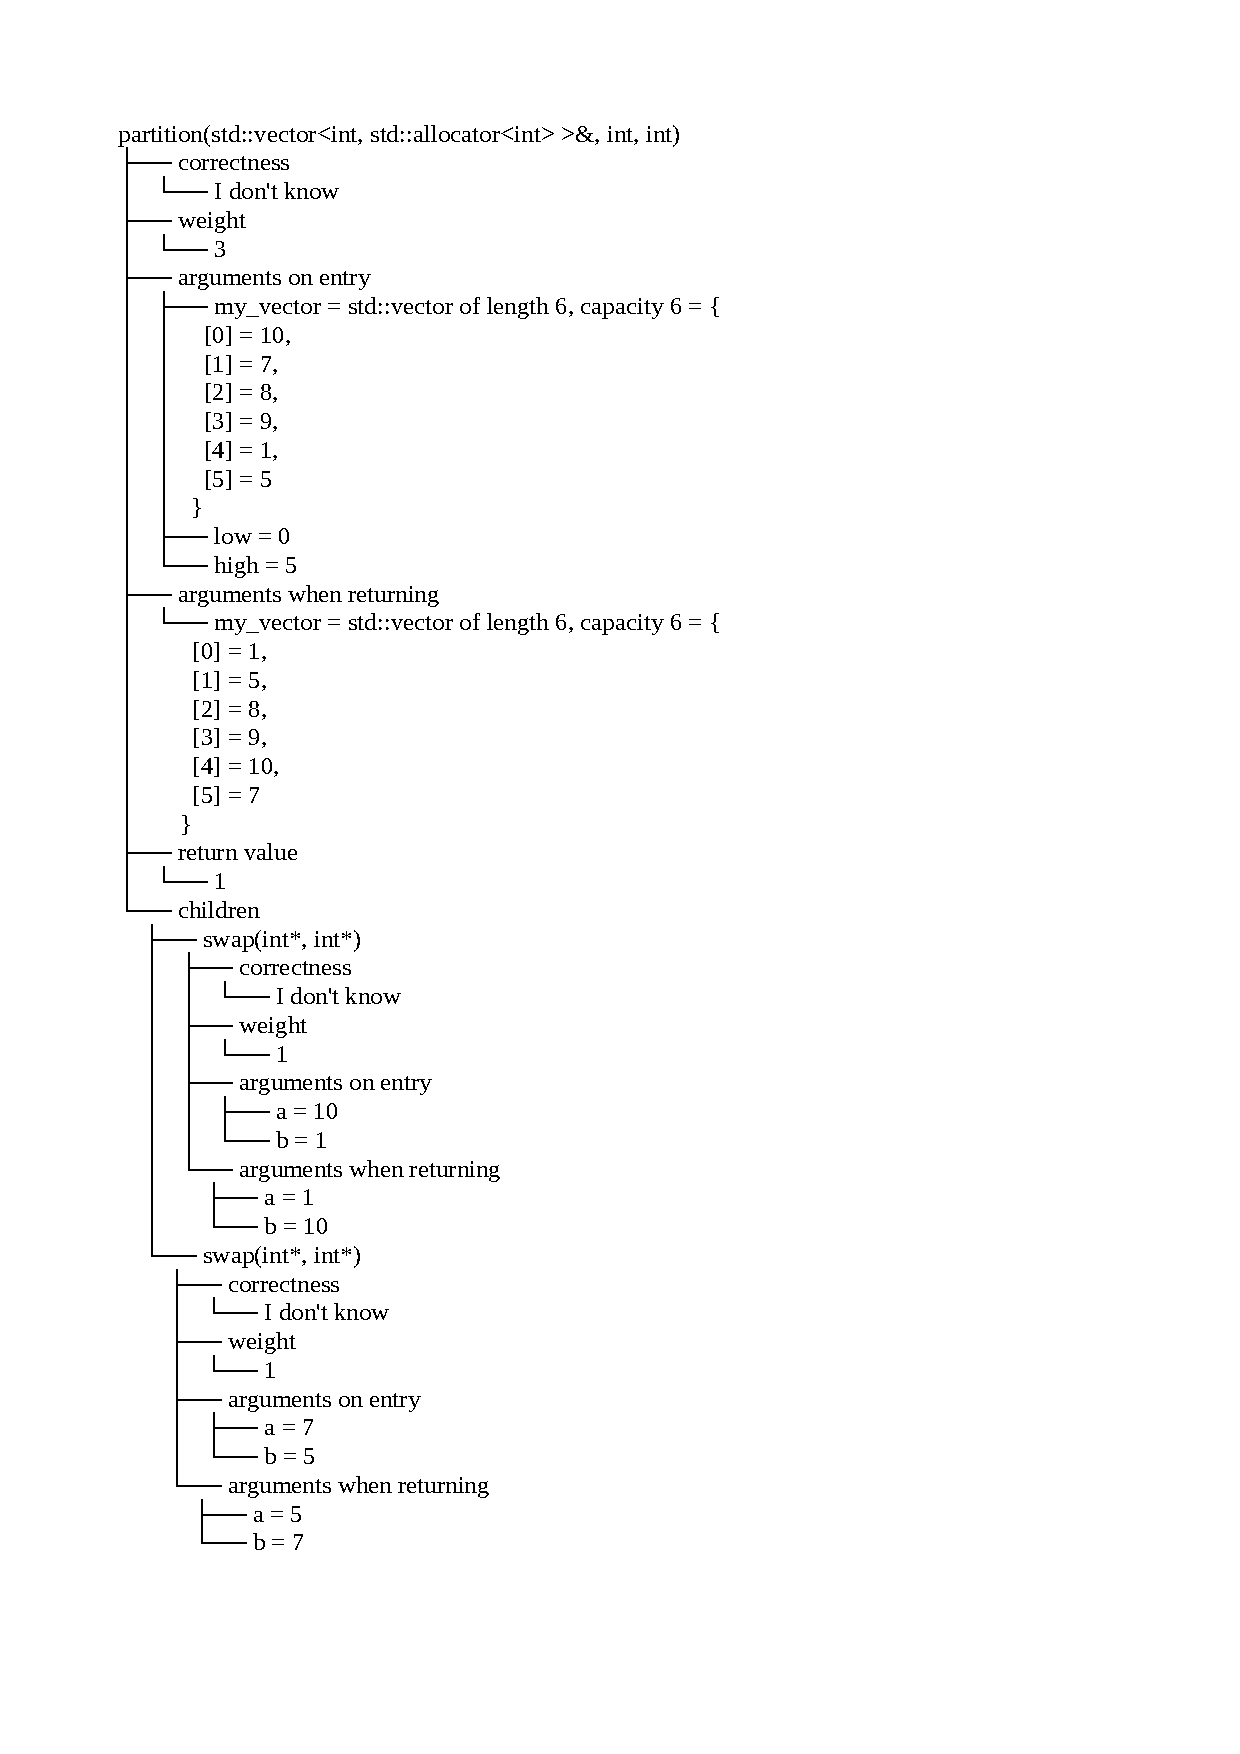
\includegraphics[width=\textwidth,height=\textheight,keepaspectratio]{Imagenes/Vectorial/partitionTree.pdf}
\end{figure}

\begin{definition}[Intended interpretation]
The intended interpretation of a function or method \(f\) given an input set \(I\), denoted \(\mathit{II}_f(I) \to O'\), is a mapping from \(I\) to \(O'\), where \(O'\) is the expected result of executing \(f(I)\).
\end{definition}
\begin{definition}[Wrong node]
A wrong node \(n_{wrong} = f(I) \to O\) is a node that is not equal to its intended interpretation, \(\mathit{II}_f(I) \to O'\).
\end{definition}
\begin{definition}[Correct node]
A correct node is a node that is equal to its intended interpretation.
\end{definition}
\begin{definition}[Buggy node]
A buggy node is a wrong node in which all its children are correct nodes. 
\end{definition}
\theoremstyle{definition}
\begin{exmp}
Figure~\ref{fig:intendedInterpretationSwap} is the intended interpretation of swap \(\mathit{II}_{swap}(I) \to O'\), \(I\) being two pointers pointing to 10 and 1 respectively.
On the other hand, Figure~\ref{fig:buggySwap} is the node \(n_{swap}(I) \to O\) of the execution of swap given the same arguments.
Since \(O'\neq O\) (note that in Figure \ref{fig:buggySwap} swap returns \(a = 10\) and \(b = 1\), whereas in Figure~\ref{fig:intendedInterpretationSwap} \texttt{swap} returns \(a = 1\) and \(b = 10\)), we can say that \(n_{swap}\) is a buggy node, and therefore there is a bug in the function \(swap\).

\begin{figure}[h]
\caption{Intended interpretation of swap function given pointer a to 10 and pointer b to 1}
\label{fig:intendedInterpretationSwap}
\begin{verbatim}
swap(int*, int*)
├── arguments on entry
│   ├── a = 10
│   └── b = 1
└── arguments when returning
    ├── a = 1
    └── b = 10
\end{verbatim}
\end{figure}

\begin{figure}[h]
\caption{Buggy node representing the execution of swap}
\label{fig:buggySwap}
\begin{verbatim}
swap(int*, int*)
├── correctness
│   └── no
├── weight
│   └── 1
├── arguments on entry
│   ├── a = 10
│   └── b = 1
└── arguments when returning
    ├── a = 10
    └── b = 1
\end{verbatim}
\end{figure}

\end{exmp}

\begin{definition}[Detected errors]
When our debugger returns a buggy node \(n_{buggy} = f(I) \to O\), an error in the definition of \(f\) has been detected. 

\end{definition}
\newtheorem{theorem}{Theorem}
\begin{theorem}[Completeness]
%Completion theorem
Let \(T = (N,E,W,M)\) be a weighted marked execution tree and S the top down strategy.
If S receives T as input, it always terminates, producing either \(\bot\) if the root node \(T\) is correct \todo{A qué te refieres?} or \(n'\in N\) otherwise.
\end{theorem}
\begin{proof}
See \cite{DeclarativeErrorDiagnosis}.
\end{proof}
\begin{theorem}[Soundness]
%Soundness theorem
Let \(T = (N,E,W,M)\) be a weighted marked execution tree, F a total function such that for every node \(n\in N\) there is a function or method \(f\) such that \(F:n\to f\), \(\mathit{II}\) a total function such that for every function or method \(f\in F\) there is an intended interpretation \(II_f\) such that \(\mathit{II}:f\to II_f\), G\todo[color=green]{No se que letra elegir aqui. Lo que quiero conseguir es la tupla de entrada a la funcion} a total function such that for every node \(n\in N\) there is 3-tuple of inputs \(I\) such that \(G:n\to I\) and S the top down strategy.
\begin{itemize}
    \item If S receives T as input and returns a node \(n'\), then \(n'\in N\), \(F(n') = f'\), \(\mathit{II}(f') = II_{f'}\), \(G(n') = I\), and \(II_{f'}(I)\neq f'(I)\).
    \item If S receives T as input and returns \(\bot\), then \(\forall n'\in N\), \(F(n') = f'\), \(\mathit{II}(f') = II_{f'}\), \(G(n') = I\), and \(II_{f'}(I) = f'(I)\).
\end{itemize}
\end{theorem}\todo{Si esto es corrección debes decir que si se detecta un nodo buggy entonces corresponde a una función que realmente contiene un bug, ¿es eso lo que dices?}\todo[color=green]{Sí, en el segundo caso quiero decir que si no encuentra nada, (porque el nodo raiz es correcto), significa que todos las funciones se adecuan a sus respectivas interpretaciones pretendidas con los inputs dados}
\begin{proof}
See \cite{DeclarativeErrorDiagnosis}.
\end{proof}


\chapter{Tool description}
\label{cap:toolDescription}
DDC consists of approximately 900 lines of mostly statically typed Python, which can be found in the following url: \url{https://github.com/RCoeurjoly/DDC/blob/main/declarative_debugger.py}.
%
It is loaded into rr through the source command, which itself can be put inside a \verb|.gdbinit| file.

In the following section, we will go through two usage scenarios:
\begin{itemize}
    \item Bug finding.
    \item Using test cases as oracles to reduce tree size.
\end{itemize}

Then, we will explain the implementation of the tool and the most important design decisions made. 
%
Lastly, we will list all commands provided by the tool.

\section{Usage scenarios}
This section describes two usage scenarios with DDC.
We will explain which commands should be executed and the expected output.
\todo{Algo de texto}

\subsection{Bug finding}
The execution of the code in Figure~\ref{lst:unexpectedQuicksortSource} results in an unexpected output, \(\{10, 5, 1, 7, 8, 9\}\), which is not sorted.
It uses the implementations of functions \verb|quickSort|, \verb|partition|, and \verb|swap| defined in Figure~\ref{lst:quicksortFunctions}.
\begin{lstlisting}[language=C++, caption={Code that results in unexpected output}, frame=tb, label={lst:unexpectedQuicksortSource}]
#include <quicksort.h>

int main()
{
  std::vector<int> my_vector{ 10, 7, 8, 9, 1, 5 };
  quickSort(my_vector, 0, my_vector.size()-1);
  std::cout << "Sorted vector: " << std::endl;
  print_vector(my_vector);
  return 0;
}
\end{lstlisting}

\begin{lstlisting}[language=C++, caption={quickSort, partition and swap implementations}, frame=p, label={lst:quicksortFunctions}]
#include <iostream>
#include <vector>

void swap(int* a, int* b)
{
  if (*a != 10)
    std::swap(*a, *b);
}

int partition(std::vector<int> &my_vector, int low, int high)
{
  int pivot = my_vector[high];
  int i = (low - 1);
  for (int j = low; j <= high - 1; j++)
    {
      if (my_vector[j] <= pivot)
        {
          i++;
          if (i != j)
            swap(&my_vector[i], &my_vector[j]);
        }
    }
  if ((i + 1) != high)
    swap(&my_vector[i + 1], &my_vector[high]);
  return (i + 1);
}

void quickSort(std::vector<int> &my_vector, int low, int high)
{
  if (low < high)
    {
      int pi = partition(my_vector, low, high);
      quickSort(my_vector, low, pi - 1);
      quickSort(my_vector, pi + 1, high);
    }
}

void print_vector(const std::vector<int> &my_vector)
{
  for (size_t i = 0; i < my_vector.size(); i++) {
    std::cout << my_vector[i] << ' ';
  }
}
\end{lstlisting}

To begin a debugging session with the purpose of finding the cause of the error, we first have to record and replay the buggy program with \verb|rr|. This is shown in 
Figure~\ref{lst:compileRecordReplayQuicksort}.
\begin{lstlisting}[language=bash, caption={Compiling, recording and replaying quickSort}, frame=tb, label={lst:compileRecordReplayQuicksort}]
nix build
rr record ./result/bin/quicksort
rr replay
\end{lstlisting}
Once inside the \verb|rr| command prompt, we have to tell DDC in which functions we suspect the bug to reside.
To do this, we use the \verb|suspect-function| command described in \ref{command:suspect-function}\todo{A menudo pones ref pero no Figure o lo que sea, revisar. Además, Figure va con mayúscula (ha cambiado varias, pero revisar)}. In this case, we suspect the functions we defined, that is, \verb|quickSort|, \verb|partition|, and \verb|swap|. We execute the commands shown in Figure \ref{fig:suspecting-functions} in \verb|rr|.
\begin{figure}[h]
    \centering
    \caption{Setting the suspect functions}
    \label{fig:suspecting-functions}
    \begin{verbatim}
(rr) suspect-function quickSort(std::vector<int>&, int, int)
Breakpoint 1 at 0x40135e: file quicksort.h, line 44.
(rr) suspect-function partition(std::vector<int>&, int, int) 
Breakpoint 2 at 0x401256: file quicksort.h, line 20.
(rr) suspect-function swap(int*, int*) 
Breakpoint 3 at 0x401222: file quicksort.h, line 9.
(rr) info breakpoints
Num Type       Disp Enb Address         What
1   breakpoint keep y   0x40135e in quickSort(std::vector<int>&, int, int)
    add-node-to-session quickSort(std::vector<int>&, int, int)
2   breakpoint keep y   0x401256 in partition(std::vector<int>&, int, int)
    add-node-to-session partition(std::vector<int>&, int, int)
3   breakpoint keep y   0x401222 in swap(int*, int*)
    add-node-to-session swap(int*, int*)
    \end{verbatim}
\end{figure}
Note that the results of the command \verb|info breakpoints| have been simplified for display purposes.
Now we can choose the navigation strategy.
\begin{figure}[h]
    \centering
    \caption{Choosing the navigation strategy}
    \label{fig:navigationsStrategyPrompt}
    \begin{verbatim}
Please choose navigation strategy
> Top-down
  Divide and Query (Hirunkitti)
  Heaviest first
    \end{verbatim}
\end{figure}
Then, as shown in Figure \ref{fig:correctnessQuestion}, the debugger asks us about the correctness of the root node of the execution tree. This question does not have the option to change the navigation strategy, as opposed to all other correctness questions, where the options are shown in Figure \ref{fig:correctnessQuestionNonRootOptions}. 

\begin{figure}[h]
    \centering
    \caption{Correctness question of root node}
    \label{fig:correctnessQuestion}
    \begin{verbatim}
You have selected Top-down!
Is the following node correct?
quickSort(std::vector<int, std::allocator<int> >&, int, int)         
├── correctness
│   └── I don't know
├── weight
│   └── 14
├── arguments on entry
│   ├── my_vector = std::vector of length 6, capacity 6 = {
│   │     [0] = 10,
│   │     [1] = 7,
│   │     [2] = 8,
│   │     [3] = 9,
│   │     [4] = 1,
│   │     [5] = 5
│   │   }
│   ├── low = 0
│   └── high = 5
└── arguments when returning
    └── my_vector = std::vector of length 6, capacity 6 = {
          [0] = 10,
          [1] = 5,
          [2] = 1,
          [3] = 7,
          [4] = 8,
          [5] = 9
        }
> Yes
  No
  I don't know
  Trusted
    \end{verbatim}
\end{figure}

\begin{figure}[h]
    \centering
    \caption{Options to correctness question of non root node}
    \label{fig:correctnessQuestionNonRootOptions}
    \begin{verbatim}
> Yes
  No
  I don't know
  Trusted
  Change strategy
    \end{verbatim}
\end{figure}

The debugging session ends when the buggy node is found, as shown in Figure \ref{fig:buggyNodeFound}. Although we only have the granularity to say which function is buggy, we also display with what inputs the buggy function misbehaves, so that the user can create a test case that reproduces the failure.
\begin{figure}[h]
    \centering
    \caption{Buggy node found}
    \label{fig:buggyNodeFound}
    \begin{verbatim}
Buggy node found
swap(int*, int*)
├── arguments on entry
│   ├── a = 10
│   └── b = 1
└── arguments when returning
    ├── a = 10
    └── b = 1 
    \end{verbatim}
\end{figure}

\subsection{Using test cases as oracles to reduce tree size}
Now, using the same buggy program as in the previous section, we are going to gather correct nodes by executing test cases.
To do this, we first have to develop a C++ executable which uses the functions with suspect to be buggy, which we display in Figure \ref{lst:quicksortTests}.
\begin{lstlisting}[language=C++, caption=Test cases for quickSort, frame=tb, label={lst:quicksortTests}]
#include <quicksort.h>
#include <algorithm>
#include <cassert>

int main()
{
  std::vector<int> my_vector{ 0, 0, 0, 0, 0, 0 };
  const int n = 6;
  for (int i = 0; i <= 9; i++) {
    my_vector[0] = rand() % 9 + 1;
    my_vector[1] = rand() % 9 + 1;
    my_vector[2] = rand() % 9 + 1;
    my_vector[3] = rand() % 9 + 1;
    my_vector[4] = rand() % 9 + 1;
    my_vector[5] = rand() % 9 + 1;
    quickSort(my_vector, 0, n-1, "");
    if (!std::is_sorted(my_vector.begin(), my_vector.end()))
      return 1;
  }
  return 0;
}
\end{lstlisting}
In this listing, we see that we test ten vectors composed of random numbers from 0 to 9. When executing these test cases, the return code is 0, so we know that our \verb|quickSort| implementation at least works for some vectors.

Like with a buggy program, we first have to record the execution with \verb|rr|. This shell will be named \(rr_{server}\), to differentiate it from the debugging shell.
\begin{lstlisting}[language=bash, caption={Compiling, recording and replaying quickSort test cases}, frame=tb, label={lst:compileRecordReplayQuicksortTests}]
nix build .#test_quicksort
rr record ./result/tests/test_quicksort
rr replay
\end{lstlisting}
Once inside the \verb|rr| command prompt, we have to tell DDC from which functions should the correct nodes be gathered.
This can be done with the \verb|save-correct-function| command described in \ref{command:save-returning-correct-node}. In our example, we want to save correct nodes gathered from the functions we defined, that is, \verb|quickSort|, \verb|partition| and \verb|swap|. Therefore, we execute the commands shown in Figure \ref{fig:saving-correct-functions} in \verb|rr|. Again, the results of the command \verb|info breakpoints| have been simplified.
\begin{figure}[h]
    \centering
    \caption{Setting the functions from which to gather correct nodes}
    \label{fig:saving-correct-functions}
    \begin{verbatim}
(rr) save-correct-function quickSort(std::vector<int>&, int, int)
Breakpoint 1 at 0x40135e: file quicksort.h, line 44.
(rr) save-correct-function partition(std::vector<int>&, int, int) 
Breakpoint 2 at 0x401256: file quicksort.h, line 20.
(rr) save-correct-function swap(int*, int*) 
Breakpoint 3 at 0x401222: file quicksort.h, line 9.
(rr) info breakpoints
Num Type       Disp Enb Address         What
1   breakpoint keep y   0x40135e in quickSort(std::vector<int>&, int, int)
    add-node-to-correct-list quickSort(std::vector<int>&, int, int)
2   breakpoint keep y   0x401256 in partition(std::vector<int>&, int, int)
    add-node-to-correct-list partition(std::vector<int>&, int, int)
3   breakpoint keep y   0x401222 in swap(int*, int*)
    add-node-to-correct-list swap(int*, int*)
    \end{verbatim}
\end{figure}

At this point, we can use the \verb|GDB| commands \verb|start| and \verb|continue| (this last one repeatedly) to reach the end of the program.
Alternatively, we have provided the convenience command \verb|til-the-end| (see section \ref{command:til-the-end}) that has the exact same functionality.
Once we have reached the end of the program, all nodes have been collected. This can be checked by dropping into an interactive Python shell inside \verb|rr| like is shown in Figure \ref{fig:python-interactive}. To exit the Python shell, use \verb|Ctrl-D|.
\begin{figure}[h]
    \centering
    \caption{Starting an interactive Python shell inside rr}
    \label{fig:python-interactive}
    \begin{verbatim}
    (rr) python-interactive
    >>>
    \end{verbatim}
\end{figure}
Once inside the shell, we can examine the set of correct nodes. For example, we can check how many correct nodes we have gathered (see Figure \ref{fig:lengthLists}) or display any of those nodes (see Figure \ref{fig:printCorrectNode}).
\begin{figure}[h]
    \centering
    \caption{Length lists}
    \label{fig:lengthLists}
    \begin{verbatim}
    >>> len(CORRECT_NODES)
    156
    >>> len(PENDING_CORRECT_NODES)
    0
    \end{verbatim}
\end{figure}

\begin{figure}[h]
    \centering
    \caption{Printing a correct node}
    \label{fig:printCorrectNode}
    \begin{verbatim}
>>> print_tree(CORRECT_NODES[0])
partition(std::vector<int, std::allocator<int> >&, int, int)
├── arguments on entry                                      
│   ├── my_vector = std::vector of length 6, capacity 6 = {                 
│   │     [0] = 2,                                                                                           
│   │     [1] = 8,                     
│   │     [2] = 1,                     
│   │     [3] = 8,                     
│   │     [4] = 6,                     
│   │     [5] = 8                     
│   │   }                      
│   ├── low = 0                              
│   └── high = 5                        
├── arguments when returning                       
│   └── my_vector = std::vector of length 6, capacity 6 = {           
│         [0] = 2,
│         [1] = 8,
│         [2] = 1,
│         [3] = 8,
│         [4] = 6,
│         [5] = 8
│       }
└── return value
    └── 5
    \end{verbatim}
\end{figure}
Once all correct nodes have been collected, we have to start the debugging session of our buggy program with a separate \verb|rr| execution (see Figure \ref{lst:compileRecordReplayQuicksort}), which we will call \(rr_{client}\), and collect the correct nodes already gathered from \(rr_{server}\). This has to be done with the command \verb|listen-for-correct-nodes}| (see \ref{command:listen-for-correct-nodes}). 

Now we are ready to send the correct nodes from \(rr_{server}\) to \(rr_{client}\). This is done with the command \verb|send-correct-nodes| (see section \ref{command:send-correct-nodes}).
In \(rr_{server}\) we can see that nodes are being sent, like shown in Figure \ref{fig:sendingNode}.
\begin{figure}[h]
    \centering
    \caption{Sending nodes to client}
    \label{fig:sendingNode}
    \begin{verbatim}
    Sending node n# 87
    \end{verbatim}
\end{figure}
Likewise, in \(rr_{client}\) we can see that nodes are being received, like shown in Figure \ref{fig:receivingNode}.
\begin{figure}[h]
    \centering
    \caption{Receiving nodes from server}
    \label{fig:receivingNode}
    \begin{verbatim}
    Connected by ('127.0.0.1', 51126)
    \end{verbatim}
\end{figure}

\begin{figure}[p]
\centering
    \caption{Zoomable tree of buggy quickSort after correct node elimination}
    \label{fig:buggyTreeAfter}
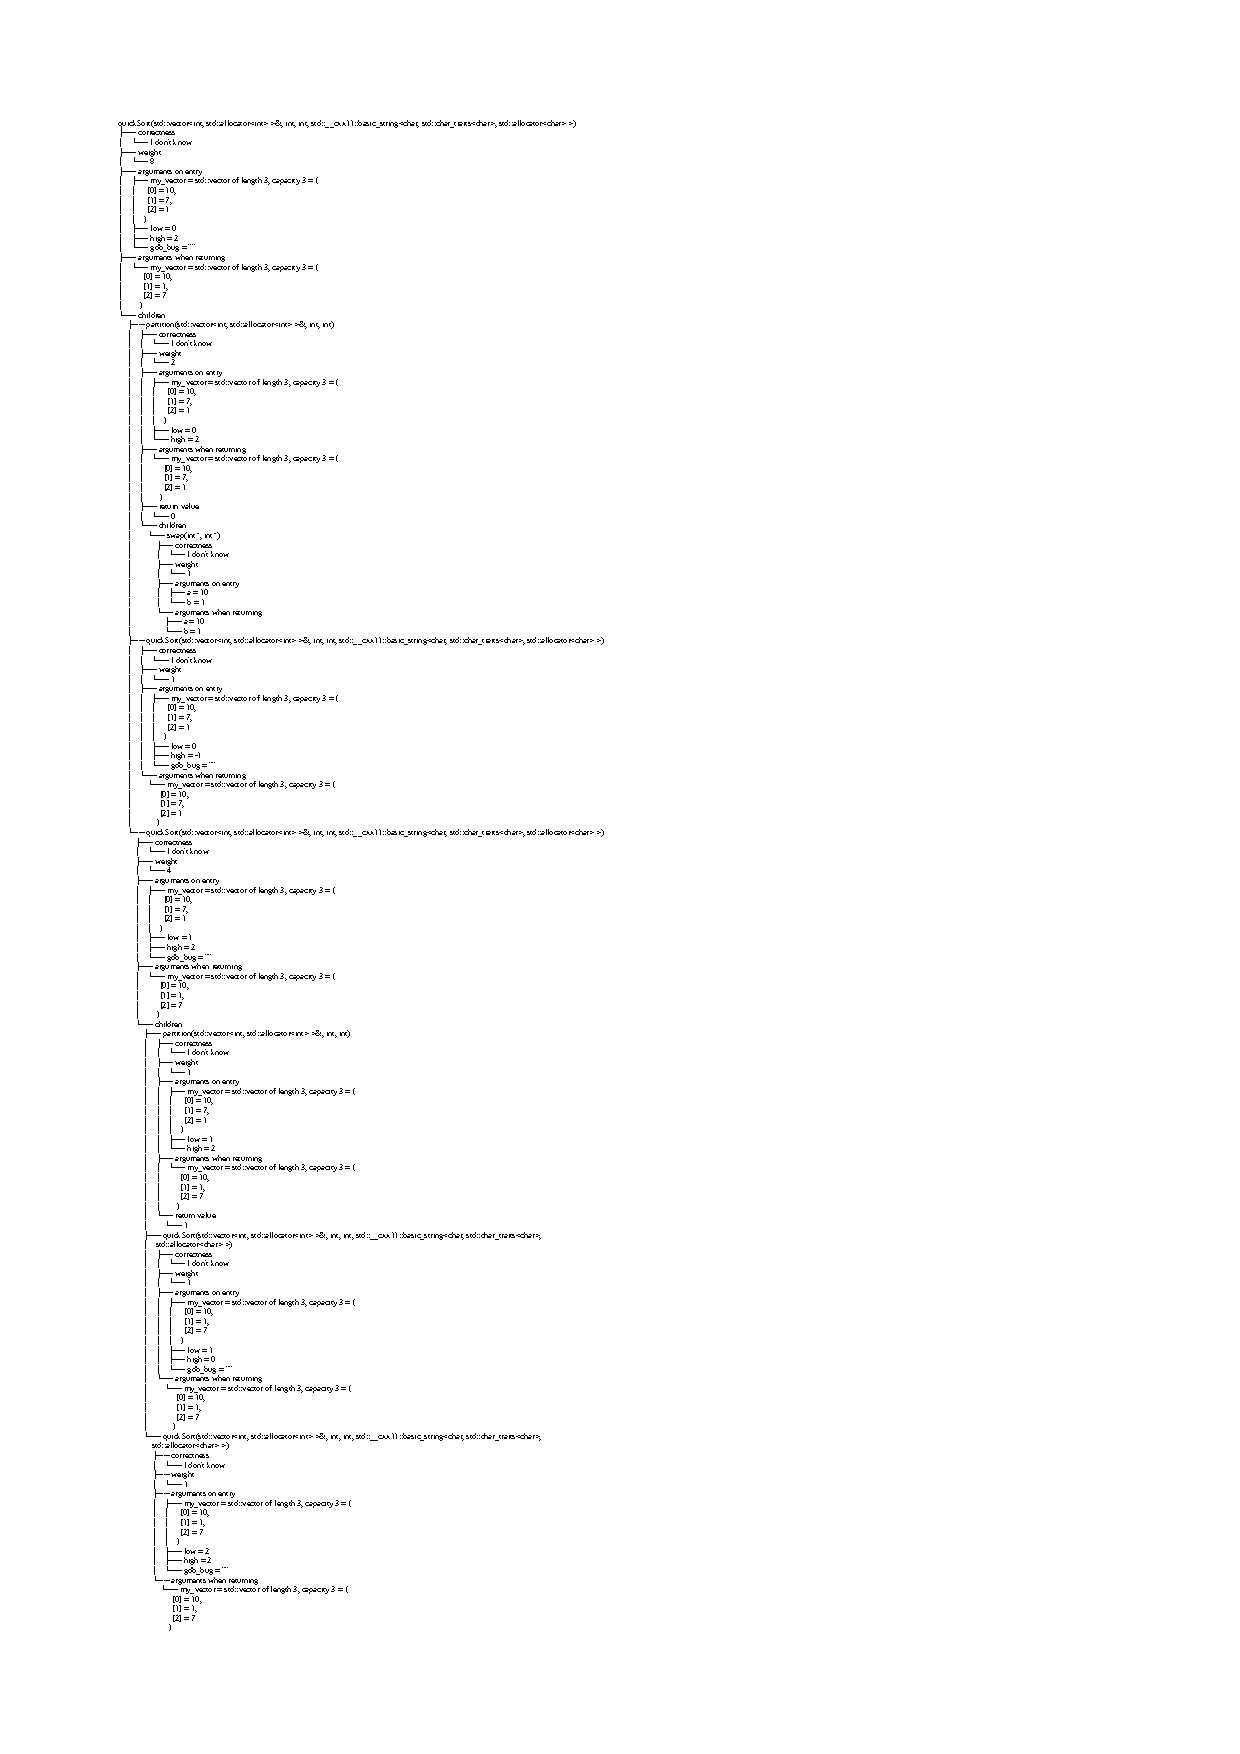
\includegraphics[width=\textwidth,height=\textheight,keepaspectratio]{Imagenes/Vectorial/buggySwapRemoved.pdf}
\end{figure}

\begin{figure}[p]
\centering
    \caption{Zoomable tree of buggy quickSort before correct node elimination}\todo{Esto es imposible verlo}
    \label{fig:buggyTreeBefore}
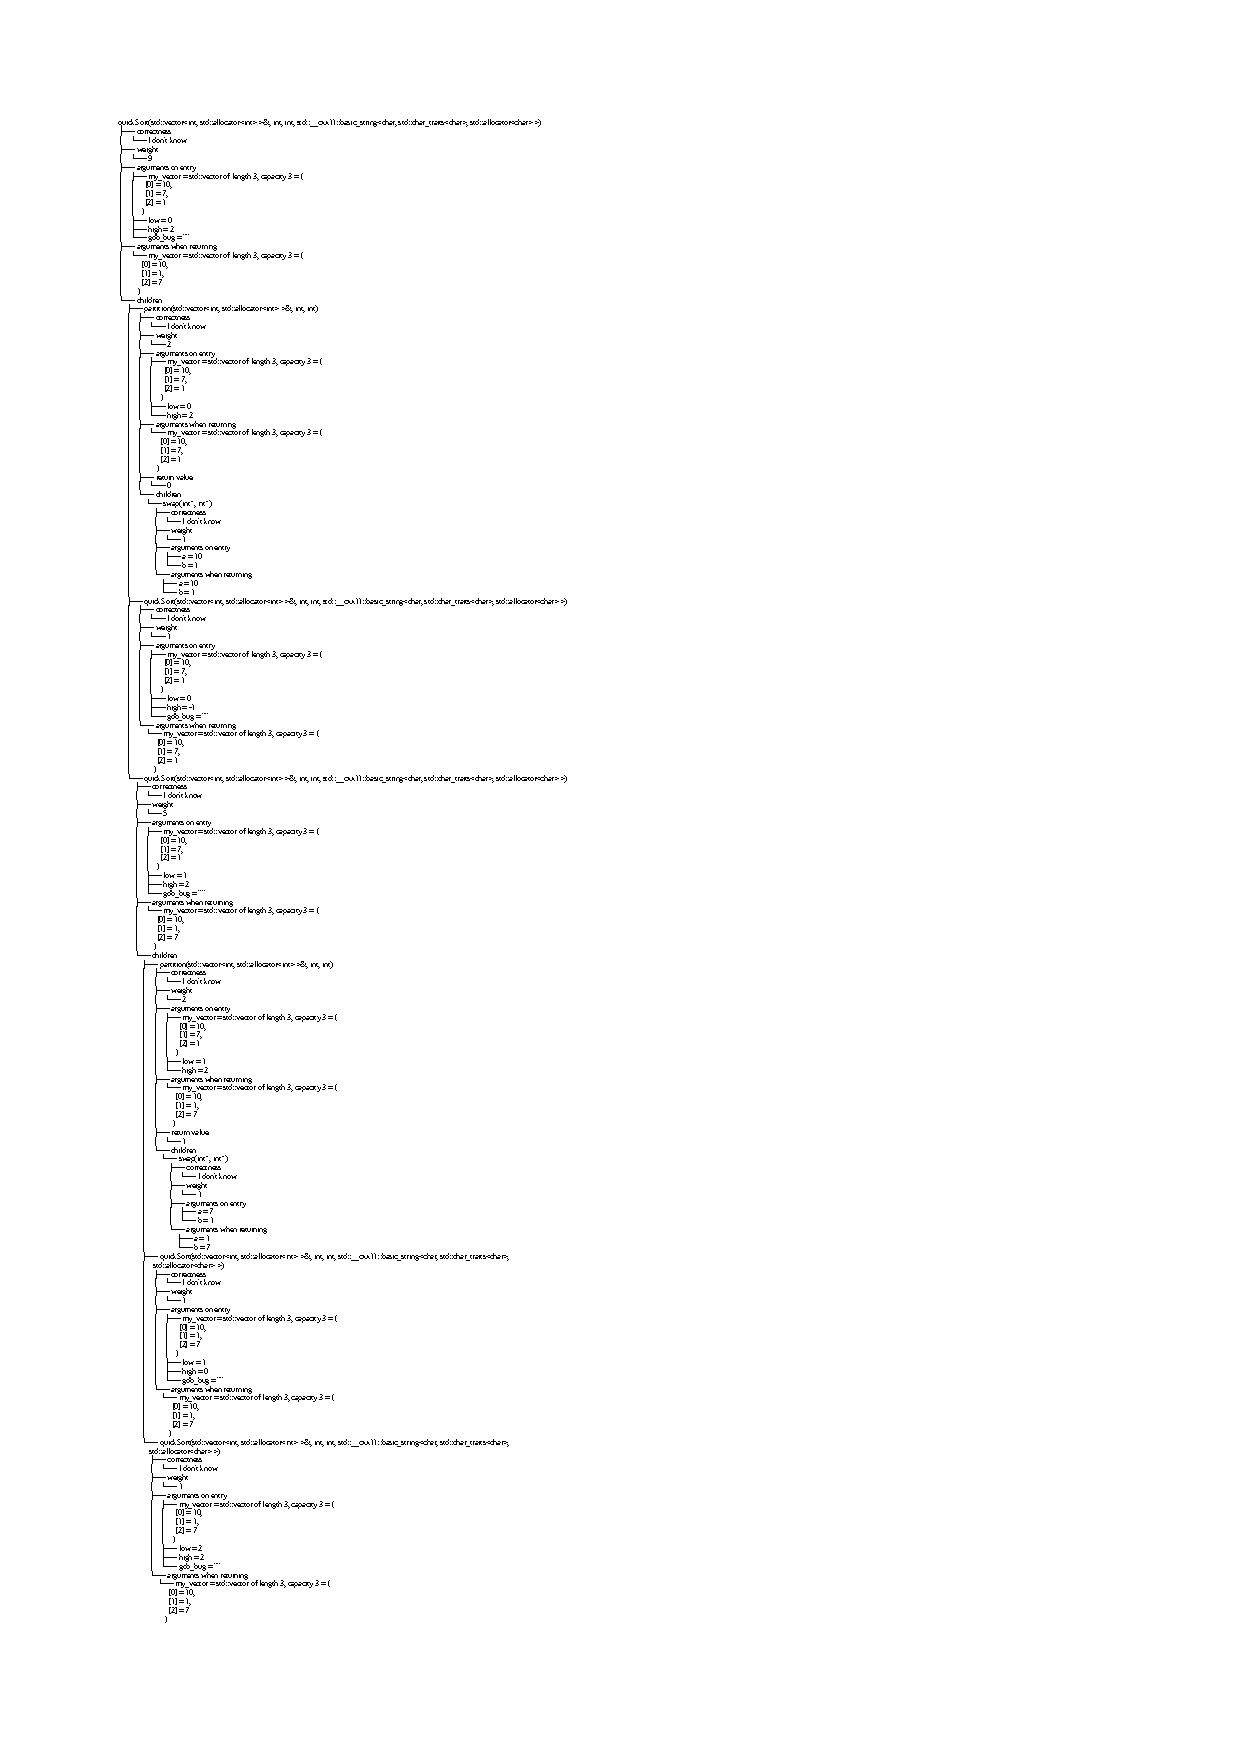
\includegraphics[width=\textwidth,height=\textheight,keepaspectratio]{Imagenes/Vectorial/buggy.pdf}
\end{figure}
%\begin{figure}
%\centering
%\caption{Correct node removed from debugging tree}
%\label{fig:removedNode}
%\begin{verbatim}
%swap(int*, int*)
%├── arguments on entry
%│   ├── a = 7
%│   └── b = 1
%└── arguments when returning
%    ├── a = 1
%    └── b = 7
%\end{verbatim}
%\end{figure}
\begin{figure}[p]
\centering
    \caption{Prueba}
    \label{fig:correctNodeRemoved}
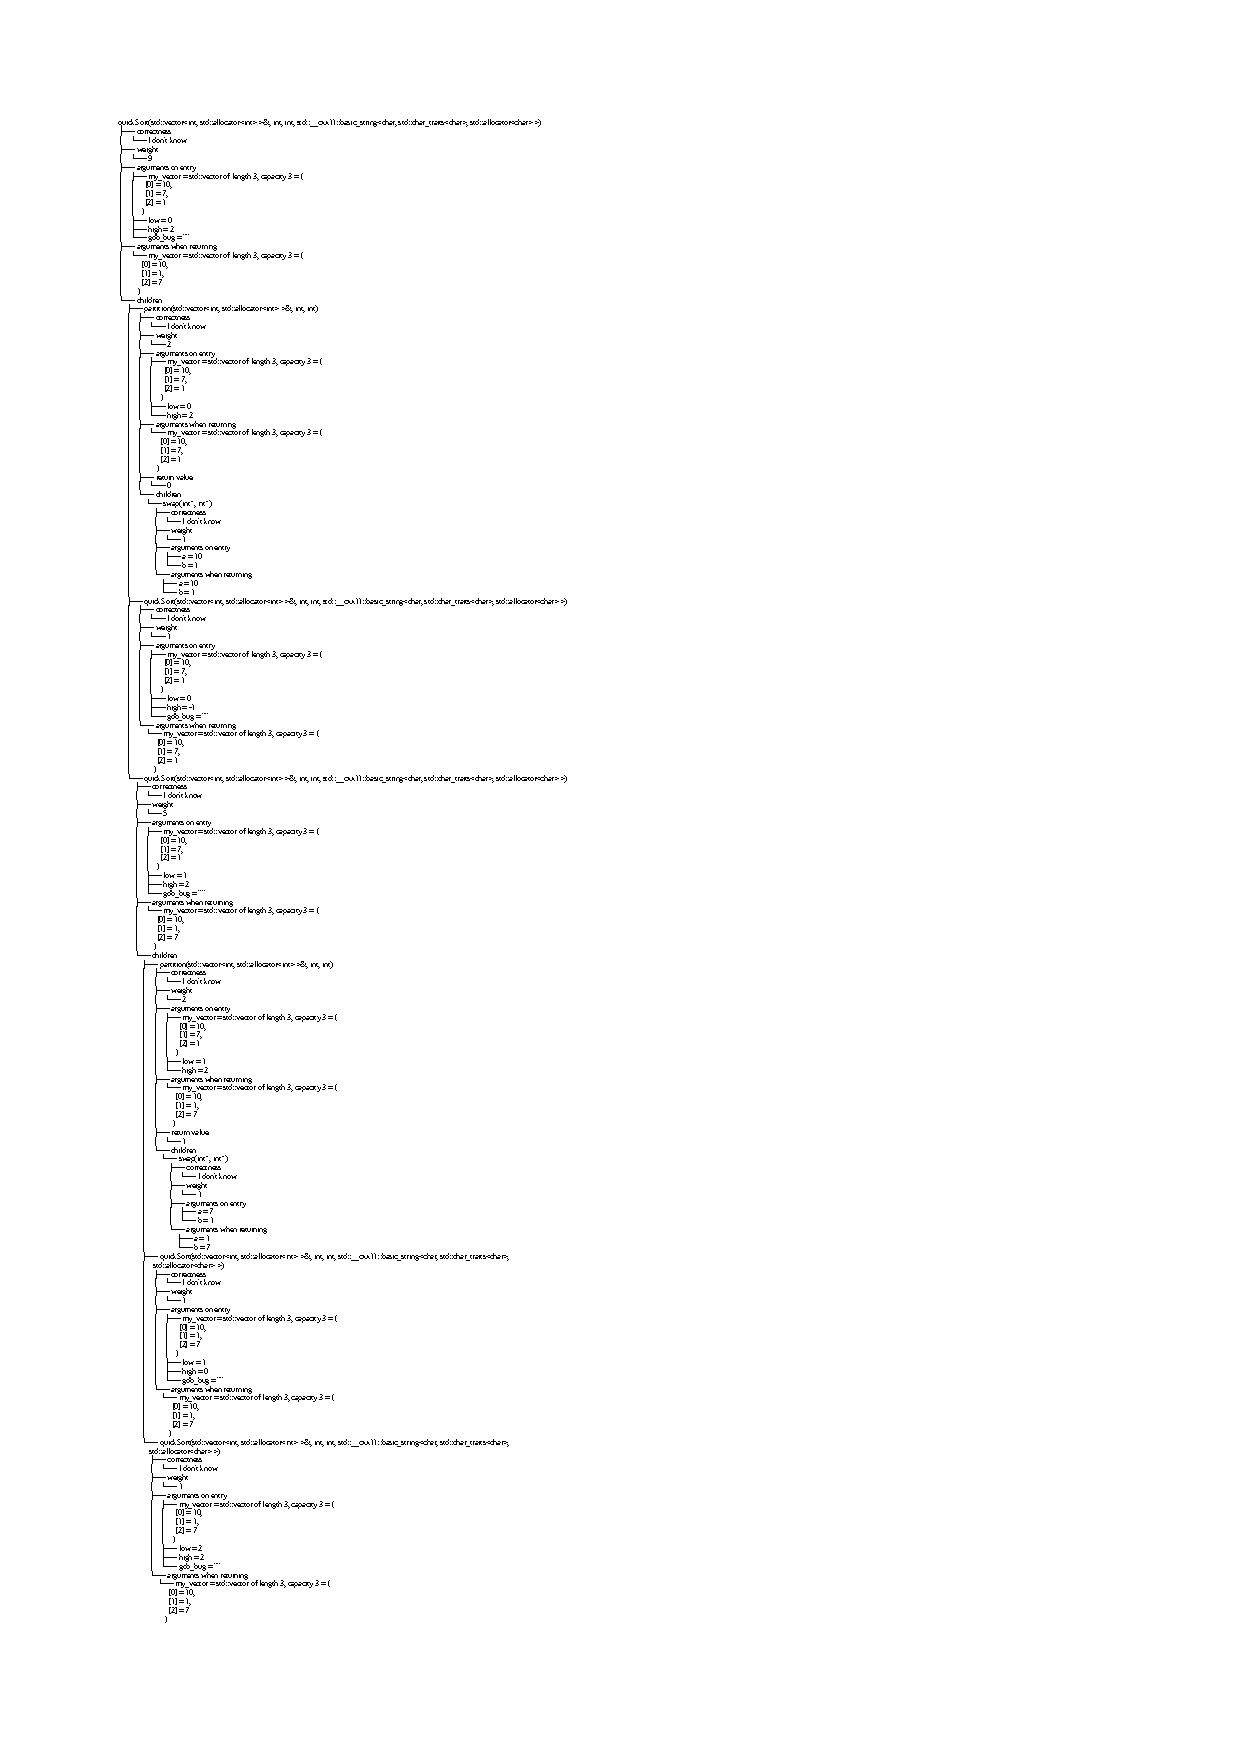
\includegraphics[width=\textwidth,height=\textheight,keepaspectratio]{Imagenes/Vectorial/buggy.pdf}
\end{figure}
If we now start the debugging session (after setting the suspect functions like demonstrated in (insert reference)), we see that the WMET has 8 nodes (see Figure \ref{fig:buggyTreeAfter}) instead of 9 (see Figure \ref{fig:buggyTreeBefore}). This is because a swap node has been removed, more specifically, the node in Figure \ref{fig:correctNodeRemoved}.


This node has been removed from the debugging tree because it appeared in a test case, therefore the debugger has deduced that this computation is correct.




\section{Implementation}
In this section we detail and justify the most important design decisions made while developing DDC.
\subsection{Tree building}
The tree is stored as the attribute \verb|node| of the global variable \verb|MY_DEBUGGING_SESSION|.
\begin{lstlisting}[language=Python, caption=DebuggingSession class and global object]
class DebuggingSession:
    def __init__(self) -> None:
        self.node = None
        self.started = False
        self.is_tree_built = False

    def start(self) -> None:
        self.started = True

    def tree_built(self) -> None:
        self.is_tree_built = True

MY_DEBUGGING_SESSION = DebuggingSession()
\end{lstlisting}
The \verb|Node| class is a recursive data structure, since it has an attribute called \verb|children| which is a list of \verb|Node|s.
\subsubsection{Adding a node to the tree}
We add a node to the debugging tree once we hit a breakpoint.
The node is added to the last position of the tree.
At that moment we add the 3-tuple of inputs to the node.
\subsubsection{Finishing a node}
When the finish breakpoint of a certain function it hit, we add the 4-tuple of outputs.
\subsubsection{Finishing the tree building process}
The tree is considered built if one of the following happens:
\begin{itemize}
    \item A final point has been hit
    \item The program has finished
    \item The root node has been completed
\end{itemize}
\subsection{Tree transformations}
After having the WMET built, we apply all tree transformations available.
\begin{lstlisting}[language=Python, caption=Applying all tree transformations]
tree_transformations = [simplified_tree_compression]
for tree_transformation in tree_transformations:
    apply_tree_transformations(MY_DEBUGGING_SESSION.node,
                               tree_transformation)
\end{lstlisting}
A tree transformation is an algorithm that receives a WMET an returns another WMET.
DDC implements for the simplified tree compression algorithm, which is described next.
\subsubsection{Simplified tree compression}
The simplified tree compression algorithm consists in two steps:
\begin{itemize}
    \item Compressing the root of the WMET if it can be compressed.
    \item Compressing each of the children nodes of the root of the WMET if they can be compressed.
\end{itemize}
\begin{lstlisting}[language=Python, caption=Simplified tree compression algorithm]
def simplified_tree_compression(marked_execution_tree: Node, position: List[int]) -> None:
    compress, nodes_to_compress = can_node_be_compressed(marked_execution_tree)
    if compress:
        compress_node_in_position_and_update_weight(marked_execution_tree,
                                                    position,
                                                    nodes_to_compress)
    for index, child_node in enumerate(marked_execution_tree.children):
        compress, nodes_to_compress = can_node_be_compressed(child_node)
        if compress:
            position.append(index)
            compress_node_in_position_and_update_weight(marked_execution_tree,
                                                        position,
                                                        nodes_to_compress)
\end{lstlisting}
Given a WMET, we can compress nodes if:
\begin{itemize}
    \item The root node has only one child node.
    \item The root and child nodes function names are the same.
\end{itemize}
To check if a node can be compressed we use the following recursive function, which takes a node as an argument and returns a 2-tuple, whose elements are:
\begin{itemize}
    \item bool: True if the node can be compressed. False otherwise.
    \item int: If the node can be compressed, number of nodes to compress. Zero Otherwise. 
\end{itemize}
This algorithm searches for the longest compression possible.
\begin{lstlisting}[language=Python, caption=Checking if node can be compressed]
def can_node_be_compressed(marked_execution_tree: Node) -> Tuple[bool, int]:
    if len(marked_execution_tree.children) != 1:
        return False, 0
    if marked_execution_tree.children[0].function_name != marked_execution_tree.function_name:
        return False, 0
    _, downstream_length = can_node_be_compressed(marked_execution_tree.children[0])
    return True, downstream_length + 1
\end{lstlisting}

Given a WMET and a number of nodes to compress \(n\), the compress node is composed of:
\begin{itemize}
    \item The 3-tuple of inputs to the root node.
    \item The 4-tuple of outputs of the node in depth \(n\) of the WMET.
    \item The name of the root node with an indication that corresponds to \(n\) compressed nodes.
\end{itemize}
This is implemented in the following function:
\begin{lstlisting}[language=Python, caption=Compression node]
def compress_node(marked_execution_tree: Node, nodes_to_compress: int) -> Node:
    head_node = marked_execution_tree
    tail_node = marked_execution_tree
    for _ in range(nodes_to_compress):
        tail_node = tail_node.children[0]
    compressed_node = tail_node
    compressed_node.arguments_on_entry_tree = head_node.arguments_on_entry_tree
    compressed_node.global_variables_on_entry_tree = head_node.global_variables_on_entry_tree
    compressed_node.object_state_on_entry_tree = head_node.object_state_on_entry_tree
    compressed_node.function_name = head_node.function_name + "^" + str(nodes_to_compress + 1)
    return compressed_node
\end{lstlisting}

The following function substitutes the compress node in place and updates the weights upstream.
\begin{lstlisting}[language=Python, caption=How to determine if a buggy node has been found]
def compress_node_in_position_and_update_weight(marked_execution_tree: Node,
                                                position: List[int],
                                                nodes_to_compress: int) -> None:
    get_node_from_position(
        marked_execution_tree,
        position).deepcopy(
            compress_node(
                get_node_from_position(marked_execution_tree,
                                       position), nodes_to_compress))
    update_nodes_weight(marked_execution_tree, position, - nodes_to_compress)
    get_node_from_position(marked_execution_tree, position).weight += nodes_to_compress
\end{lstlisting}
\subsection{General debugging algorithm}
The general debugging algorithm takes two arguments:
\begin{itemize}
    \item The WMET.
    \item A navigation strategy.
\end{itemize}
It returns either a buggy node or \(\bot\).
It consists of loop, from which we exit if the WMET is empty or a buggy node has been found.
To determine if a node has been found we have to check that the WMET consists of an unique incorrect node.
\begin{lstlisting}[language=Python, caption=How to determine if a buggy node has been found]
def buggy_node_found(marked_execution_tree: Node) -> bool:
    return (marked_execution_tree.iscorrect == Correctness.NO
            and len(marked_execution_tree.children) == 0)
\end{lstlisting}
Once inside the loop, first we select the node to be asked about by means of the strategies, which are explained in \hyperref[implementation:Strategies]{Section Strategies}.
We then ask the user about the node. One of the options available to the user is to change strategy. If this is chosen, we ask the user her preferred strategy and continue the execution of the loop.
\begin{lstlisting}[language=Python, caption=Function to ask about node]
def ask_about_node_with_extra_functionality(node: Node) -> Union[Correctness, ExtraFunctionality]:
    print("Is the following node correct?")
    print_tree(node.get_tree(get_children=False))
    correctness_options = ["Yes", "No", "I don't know", "Trusted"]
    total_options = correctness_options + [
        "Change strategy"]
    terminal_menu = TerminalMenu(total_options)
    menu_entry_index = terminal_menu.show()
    answers_dict = {
        "Yes": Correctness.YES,
        "No": Correctness.NO,
        "I don't know": Correctness.IDK,
        "Trusted": Correctness.TRUSTED,
        "Change strategy": ExtraFunctionality.CHANGE_STRATEGY
    }
    return answers_dict[total_options[menu_entry_index]]
\end{lstlisting}

If no change in strategy is required, we execute the adequate action corresponding to the correctness answer (see \hyperref[implementation:correctnessAnswers]{Section User answers to correctness questions}) and continue the execution of the loop.

\begin{lstlisting}[language=Python, caption=General debugging algorithm implementation]
def general_debugging_algorithm(marked_execution_tree: Optional[Node],
                                strategy: Callable[[Node,
                                                    List[int]],
                                                   Tuple[Node,
                                                         bool,
                                                         List[int]]]
                                ) -> Optional[Node]:
    while (marked_execution_tree is not None
           and not and not buggy_node_found(marked_execution_tree)):
        assert marked_execution_tree.iscorrect == Correctness.NO
        selected_node, found, position = select_node(marked_execution_tree,
                                                     strategy)
        assert found
        assert selected_node.weight > 0
        answer = ask_about_node_with_extra_functionality(selected_node)
        if answer == ExtraFunctionality.CHANGE_STRATEGY:
            strategy = strategies_dict[choose_strategy()]
            continue
        selected_node.iscorrect = answer
        function_name = selected_node.function_name
        node_tree = selected_node.get_tree(get_children=False,
                                           get_weight=False,
                                           get_correctness=False)
        if answer == Correctness.NO:
            marked_execution_tree = selected_node
            continue
        elif answer in [Correctness.YES,
                        Correctness.IDK,
                        Correctness.TRUSTED]:
            # Remove the node and remove the weight from all its parents
            remove_node_and_update_tree(marked_execution_tree,
                                        position)
        if answer == Correctness.YES:
            remove_correct_node_from_tree(marked_execution_tree,
                                          node_tree)
        elif answer == Correctness.TRUSTED:
            remove_trusted_node_from_tree(marked_execution_tree,
                                          function_name)
    return marked_execution_tree
\end{lstlisting}
\subsection{Navigation strategies}
\label{implementation:Strategies}
A navigation strategy is an algorithm that takes a WMET and returns a node.
In the implementation we also need to keep track of the position of the current node, since Top-down is a recursive algorithm.

To ease the task of adding more strategies to DDC, we implemented a wrapper to the strategies.
\begin{lstlisting}[language=Python, caption=Select node implementation]
def select_node(marked_execution_tree: Node,
                strategy: Callable[[Node, List[int]],
                                   Tuple[Node, bool, List[int]]]) -> Tuple[Node, bool, List[int]]:
    return strategy(marked_execution_tree, [])
\end{lstlisting}
\subsubsection{Top-down}
Top-down is a recursive algorithm, which searches for the first node whose correctness is unknown. 
\begin{lstlisting}[language=Python, caption=Top-down strategy implementation]
def top_down_strategy(marked_execution_tree: Node,
                      position: List[int]) -> Tuple[Optional[Node], bool, List[int]]:
    """Search for closest undefined node.
    Returns:
    Found: bool
    Node
    Position: list of int
    """
    if marked_execution_tree.iscorrect == Correctness.IDK:
        return marked_execution_tree, True, position
    for index, child in enumerate(marked_execution_tree.children):
        tmp_marked_execution_tree, found, tmp_position = top_down_strategy(child, position)
        if found:
            tmp_position.append(index)
            return tmp_marked_execution_tree, found, tmp_position
    return None, False, []
\end{lstlisting}
\subsubsection{Divide and Query (Hirunkitti)}
In Divide and Query (Hirunkitti), we select the child node whose weight is the closest to half of the root node weight.
\begin{lstlisting}[language=Python, caption=Divide and Query (Hirunkitti) strategy implementation]
def divide_and_query_hirunkitti_strategy(marked_execution_tree: Node,
                                         position: List[int]) -> Tuple[Node, bool, List[int]]:
    assert len(marked_execution_tree.children) > 0
    pivot = marked_execution_tree.weight/2
    distance = marked_execution_tree.weight/2
    choosen_node = marked_execution_tree
    position = []
    for index, child in enumerate(marked_execution_tree.children):
        if abs(child.weight - pivot) < distance:
            distance = abs(child.weight - pivot)
            choosen_node = child
            position = [index]
    return choosen_node, True, position
\end{lstlisting}
\subsubsection{Heaviest first}
In heaviest first, we select the child node whose weight is the heaviest.
\begin{lstlisting}[language=Python, caption=Heaviest first strategy implementation]
def heaviest_first_strategy(marked_execution_tree: Node,
                            position: List[int]) -> Tuple[Node, bool, List[int]]:
    assert len(marked_execution_tree.children) > 0
    heaviest_weight = 0
    for index, child in enumerate(marked_execution_tree.children):
        if child.weight > heaviest_weight:
            heaviest_weight = child.weight
            choosen_node = child
            position = [index]
    return choosen_node, True, position
\end{lstlisting}
\subsection{User answers to correctness questions}
\label{implementation:correctnessAnswers}
When asked about the correctness of a node, the user has the possibility of answering (i) I don't know, (ii) Yes, (iii) No or (iv) Trusted.
We choose the next node and/or prune the debugging tree depending on the answer
\subsubsection{I don't know}
If the user does not know if the node is correct, we remove it from the WMET and continue the debugging session. 
\subsubsection{Yes}
If the node is deemed correct by the user, we remove it from the WMET and all other nodes equal to the correct node.
\begin{lstlisting}[language=Python, caption=Correct node action]
def remove_correct_node_from_tree(marked_execution_tree: Node, node_tree: Node):
    # Remove nodes with the same node_tree and remove the weight from all its parents
    while True:
        _, found, position = find_node_with_node_tree(marked_execution_tree, [], node_tree)
        if found is False:
            break               
        update_nodes_weight(marked_execution_tree,
                            position,
                            - get_node_from_position(marked_execution_tree,
                                                    position).weight)
        deleted_tree = remove_node_from_tree(marked_execution_tree, position)
        if deleted_tree:
            marked_execution_tree = None
            break
\end{lstlisting}
\subsubsection{No}
If the node is deemed incorrect by the user, we continue the navigation phase with this node as the WMET root.
\begin{lstlisting}[language=Python, caption=Incorrect node action]
if answer == Correctness.NO:
    marked_execution_tree = selected_node
\end{lstlisting}
\subsubsection{Trusted}
If the node is trusted by the user, we remove it from the WMET and all other nodes which correspond to executions of the same function of the correct node.
\begin{lstlisting}[language=Python, caption=Trusted node action]
def remove_trusted_node_from_tree(marked_execution_tree: Node, function_name: str):
    # Remove nodes with the same name and remove the weight from all its parents
    found = True
    while True:
        _, found, position = find_node_with_name(marked_execution_tree, [], function_name)
        if found is False:
            break
        update_nodes_weight(marked_execution_tree,
                            position,
                            - get_node_from_position(marked_execution_tree,
                                                     position).weight)
        deleted_tree = remove_node_from_tree(marked_execution_tree, position)
        if deleted_tree:
            marked_execution_tree = None
            break
\end{lstlisting}

\subsection{Test cases as oracles}
DDC implements the functionality of test cases as oracles with the following global variables.
\begin{lstlisting}[language=Python, caption=Global variables related to using test cases as oracles]
CORRECT_NODES: List[ComparableTree] = []
PENDING_CORRECT_NODES: List[Node] = []
\end{lstlisting}

In \verb|CORRECT_NODES| we store a list of all nodes that have finished, that is, whose functions have returned.
In \verb|PENDING_CORRECT_NODES| we store a list of all nodes that have started but not finished.

\verb|ComparableTree| is a class that derives from \verb|rich.tree|, which is the class used to present the information to the user.

The \verb|Node| class has a member function \verb|get_tree|, which returns a \verb|ComparableTree|.
For comparison with elements in the \verb|CORRECT_NODES| list, the node gets stripped of its correctness value, children and weight. 
\begin{lstlisting}[language=Python, caption={Node class method signature for getting a comparable tree}]
def get_tree(self,
             get_children: bool = True,
             get_weight: bool = True,
             get_correctness: bool = True) -> ComparableTree:
\end{lstlisting}
\begin{lstlisting}[language=Python, caption=Comparable tree class]
class ComparableTree(Tree):
    def __eq__(self, other: object) -> bool:
        return (isinstance(other, self.__class__)
            and self.to_json() == other.to_json())

    def to_json(self):
        return json.dumps(self, default=lambda o: o.__dict__,
            sort_keys=True, indent=4)
\end{lstlisting}

Once a node finishes, we search for it in the \verb|CORRECT_NODES| list. If found, we remove it from the debugging tree.
\begin{lstlisting}[language=Python, caption=Removing finished node from tree if it is correct]
if my_node.get_tree(False, False, False) in CORRECT_NODES:
    remove_node_and_update_tree(MY_DEBUGGING_SESSION.node,
                                my_node.position)
\end{lstlisting}

\section{Commands}
We now list and describe all the available commands. These can be issued inside rr. Completion for these commands is enabled, that is, if you type \verb|sus| and then \verb|TAB|, \verb|suspect-function| should appear.
The following information can also be found with \verb|help <command>|, where \verb|<command>| is one of the commands that follow.

\subsection{suspect-function}
\label{command:suspect-function}
Mandatory command used in a debugging session.

Sets a breakpoint on the location provided as argument. It also adds the command \hyperref[command:add-node-to-session]{add-node-to-session} to it.
It should be used at least once before starting the debugging session.

Arguments: location.

Location completion is enabled.
\subsection{add-node-to-session}
\label{command:add-node-to-session}
Optional command used in a debugging session.
Adds the current frame to the debugging tree.
It expects to be called on entry to a function or method.
It also creates a finish breakpoint for the current function or method, with the attach command \hyperref[command:save-returning-node]{save-returning-node}.

It can be used to create an ad hoc debugging tree.

It is used by \hyperref[command:suspect-function]{suspect-function}.

Arguments: none.
\subsection{save-returning-node}
\label{command:save-returning-node}
It saves the arguments of the function or method that just returned.
This is the command attached to finish breakpoints created with \hyperref[command:add-node-to-session]{add-node-to-session}.

For internal use only.

Arguments: none.
\subsection{final-point}
\label{command:final-point}
Optional command used in a debugging session.
Sets a breakpoint on the location provided as argument and adds the command \hyperref[command:finish-debugging-session]{finish-debugging-session} to it.
It can be used zero or more times.

Arguments: location.

Location completion is enabled.
\subsection{finish-debugging-session}
\label{command:finish-debugging-session}
Sets the Boolean variable describing that the tree has been built to true.
This command is executed when a \hyperref[command:final-point]{final-point} is reached.

Internal use only.

Arguments: none.
\subsection{start-declarative-debugging-session}
\label{command:start-declarative-debugging-session}
Mandatory command used in a debugging session.
If the debugging tree has not been built, it builds it. Otherwise, it starts to ask correctness questions to the user. 

Arguments: none.
\subsection{save-correct-function}
\label{command:save-correct-function}
Sets a breakpoint on the location provided as argument, setting as command \hyperref[command:save-returning-correct-node]{save-returning-correct-node}. Mandatory command used in gathering correct nodes.

Arguments: location.

Location completion is enabled.
\subsection{add-node-to-correct-list}
\label{command:add-node-to-correct-list}
Optional command used in gathering correct nodes.
Adds the current frame to the debugging tree.
It expects to be called on entry to a function or method.
It also sets a final breakpoint on current function or method, with the attached command \hyperref[command:save-returning-correct-node]{save-returning-correct-node}.

Arguments: none.

For internal use only.
\subsection{save-returning-correct-node}
\label{command:save-returning-correct-node}
It saves the arguments of the function or method that just returned into the appropriate node.

Arguments: none.

For internal use only.
\subsection{til-the-end}
\label{command:til-the-end}
Continues the execution of the inferior until the program is not being run.

Optional command used in gathering correct nodes.

Arguments: none.
\subsection{listen-for-correct-nodes}
\label{command:listen-for-correct-nodes}
Open a connection on localhost, port 4096, and wait for correct nodes to be sent.

Executed by the client.
Mandatory command used in gathering correct nodes.
Must be executed before calling \hyperref[command:send-correct-nodes]{send-correct-nodes} in the server.

Arguments: none.
\subsection{send-correct-nodes}
\label{command:send-correct-nodes}
Send all the correct nodes gathered from tests to the client.
Executed by the server.
The client has to have issued the \hyperref[command:listen-for-correct-nodes]{listen-for-correct-nodes} before, otherwise a ConnectionRefusedError exception is thrown.

Mandatory command used in gathering correct nodes.

Arguments: none.
\subsection{print-tree}
\label{command:print-tree}
Prints the debugging tree.
An exception is thrown if the debugging tree has not been built yet. 
Optional command that can be used in a debugging session.

Arguments: none.
\chapter{Conclusions and Future Work}
\label{cap:conclusions}

Conclusions.

By using GDB as a framework to build the declarative debugger, we have the benefit of supporting not only C++ but 
several programming languages 
(https://sourceware.org/gdb/current/onlinedocs/gdb/Supported-Languages.html).

This is done through a common Python API.

Also, by using a language with a broad amount of libraries such as Python, the user interface and execution tree representation have been easy to implement.

During the development and use of the debugger, some execution trees did not match expectations.

Upon close examination, these maybe caused by GDB.

The first is that with recursive calls

The second is that if two function calls are identical in terms of arguments passed to them, then their frames are identical.

The workaround implemented to avoid building an erroneous execution tree is two fold:

When filling information about the call on entry, the current node is appended to the list of node if:
nodes is empty
last node's frame is invalid (meaning is no longer active)
last node's frame is not a parent of current node.

When filling information about the call on return, only fill it if it is empty.

Another future line of improvements could come from the presentation of node information to the user.

Two issues have been highlighted by doing this project.

The first is arrays in C++. C++ arrays are typed as pointers to the first element of the array when passed as argument to a function. (insert screen capture of GDB to prove this)

Then, it does not seem to be a way to differentiate between pointers and arrays when working in GDB.

To surmount this difficulty, the examples programs use std::vector instead of C-style arrays.

Another issue with variable display is pointers.

Some functions, like swap(int *, int *) in the example provided, do pointer arithmetic.

Maybe we should display both the memory address pointed by the pointer and the content.

Another line of future development could be 

\section{Conclusions}
\section{Future work}
\subsection{Benchmarking overhead of building execution tree}
\subsection{Support concurrent programs}
\subsection{Test programming languages other than C++}
\subsection{Implement more strategies}
\subsection{Formally verify all algorithms}
Nagini fails
Cross hair fails (recursion too deep)
Maybe Lean to C, and the C to Python
\subsection{Generate test cases from correct nodes}
\subsection{Support for C-style arrays}
\subsection{Report GDB bugs}
\subsubsection{Wrong backtrace with recursive functions}
\subsubsection{Frame ID is the same for function call with the same arguments}
\subsection{Increase granularity in error detection}
\subsection{Increase flexibility inside a debugging session}
\subsection{Interactive/collapsible execution tree}

%%%%%%%%%%%%%%%%%%%%%%%%%%%%%%%%%%%%%%%%%%%%%%%%%%%%%%%%%%%%%%%%%%%%%%%%%%%
% Si el TFM se escribe en inglés, comentar las siguientes líneas 
% porque no es necesario incluir nuevamente las Conclusiones en inglés
% \begin{otherlanguage}{english}
% \chapter{Introduction}
\label{cap:introduction}

Introduction to the subject area. This chapter contains the translation of Chapter \ref{cap:introduccion}.










% \chapter{Conclusions and Future Work}
\label{cap:conclusions}

Conclusions and future lines of work. This chapter contains the translation of Chapter \ref{cap:conclusiones}.



% \end{otherlanguage}
%%%%%%%%%%%%%%%%%%%%%%%%%%%%%%%%%%%%%%%%%%%%%%%%%%%%%%%%%%%%%%%%%%%%%%%%%%%

%
% Bibliografía
%
% Si el TFM se escribe en inglés, editar TeXiS/TeXiS_bib para cambiar el
% estilo de las referencias
%---------------------------------------------------------------------
%
%                      configBibliografia.tex
%
%---------------------------------------------------------------------
%
% bibliografia.tex
% Copyright 2009 Marco Antonio Gomez-Martin, Pedro Pablo Gomez-Martin
%
% This file belongs to the TeXiS manual, a LaTeX template for writting
% Thesis and other documents. The complete last TeXiS package can
% be obtained from http://gaia.fdi.ucm.es/projects/texis/
%
% Although the TeXiS template itself is distributed under the 
% conditions of the LaTeX Project Public License
% (http://www.latex-project.org/lppl.txt), the manual content
% uses the CC-BY-SA license that stays that you are free:
%
%    - to share & to copy, distribute and transmit the work
%    - to remix and to adapt the work
%
% under the following conditions:
%
%    - Attribution: you must attribute the work in the manner
%      specified by the author or licensor (but not in any way that
%      suggests that they endorse you or your use of the work).
%    - Share Alike: if you alter, transform, or build upon this
%      work, you may distribute the resulting work only under the
%      same, similar or a compatible license.
%
% The complete license is available in
% http://creativecommons.org/licenses/by-sa/3.0/legalcode
%
%---------------------------------------------------------------------
%
% Fichero  que  configura  los  parámetros  de  la  generación  de  la
% bibliografía.  Existen dos  parámetros configurables:  los ficheros
% .bib que se utilizan y la frase célebre que aparece justo antes de la
% primera referencia.
%
%---------------------------------------------------------------------


%%%%%%%%%%%%%%%%%%%%%%%%%%%%%%%%%%%%%%%%%%%%%%%%%%%%%%%%%%%%%%%%%%%%%%
% Definición de los ficheros .bib utilizados:
% \setBibFiles{<lista ficheros sin extension, separados por comas>}
% Nota:
% Es IMPORTANTE que los ficheros estén en la misma línea que
% el comando \setBibFiles. Si se desea utilizar varias líneas,
% terminarlas con una apertura de comentario.
%%%%%%%%%%%%%%%%%%%%%%%%%%%%%%%%%%%%%%%%%%%%%%%%%%%%%%%%%%%%%%%%%%%%%%
\setBibFiles{%
biblio%
}

%%%%%%%%%%%%%%%%%%%%%%%%%%%%%%%%%%%%%%%%%%%%%%%%%%%%%%%%%%%%%%%%%%%%%%
% Definición de la frase célebre para el capítulo de la
% bibliografía. Dentro normalmente se querrá hacer uso del entorno
% \begin{FraseCelebre}, que contendrá a su vez otros dos entornos,
% un \begin{Frase} y un \begin{Fuente}.
%
% Nota:
% Si no se quiere cita, se puede eliminar su definición (en la
% macro setCitaBibliografia{} ).
%%%%%%%%%%%%%%%%%%%%%%%%%%%%%%%%%%%%%%%%%%%%%%%%%%%%%%%%%%%%%%%%%%%%%%

%%
%% Creamos la bibliografia
%%
\makeBib

% Variable local para emacs, para  que encuentre el fichero maestro de
% compilación y funcionen mejor algunas teclas rápidas de AucTeX

%%%
%%% Local Variables:
%%% mode: latex
%%% TeX-master: "../Tesis.tex"
%%% End:



% Apéndices
\appendix
%\chapter{Título del Apéndice A}
\label{Appendix:Key1}

Contenido del apéndice
%\chapter{Título del Apéndice B}
\label{Appendix:Key2}

%\include{Apendices/appendixC}
%\include{...}
%\include{...}
%\include{...}
\backmatter



%
% Índice de palabras
%

% Sólo  la   generamos  si  está   declarada  \generaindice.  Consulta
% TeXiS.sty para más información.

% En realidad, el soporte para la generación de índices de palabras
% en TeXiS no está documentada en el manual, porque no ha sido usada
% "en producción". Por tanto, el fichero que genera el índice
% *no* se incluye aquí (está comentado). Consulta la documentación
% en TeXiS_pream.tex para más información.
\ifx\generaindice\undefined
\else
%%---------------------------------------------------------------------
%
%                        TeXiS_indice.tex
%
%---------------------------------------------------------------------
%
% TeXiS_indice.tex
% Copyright 2009 Marco Antonio Gomez-Martin, Pedro Pablo Gomez-Martin
%
% This file belongs to TeXiS, a LaTeX template for writting
% Thesis and other documents. The complete last TeXiS package can
% be obtained from http://gaia.fdi.ucm.es/projects/texis/
%
% This work may be distributed and/or modified under the
% conditions of the LaTeX Project Public License, either version 1.3
% of this license or (at your option) any later version.
% The latest version of this license is in
%   http://www.latex-project.org/lppl.txt
% and version 1.3 or later is part of all distributions of LaTeX
% version 2005/12/01 or later.
%
% This work has the LPPL maintenance status `maintained'.
% 
% The Current Maintainers of this work are Marco Antonio Gomez-Martin
% and Pedro Pablo Gomez-Martin
%
%---------------------------------------------------------------------
%
% Contiene  los  comandos  para  generar  el índice  de  palabras  del
% documento.
%
%---------------------------------------------------------------------
%
% NOTA IMPORTANTE: el  soporte en TeXiS para el  índice de palabras es
% embrionario, y  de hecho  ni siquiera se  describe en el  manual. Se
% proporciona  una infraestructura  básica (sin  terminar)  para ello,
% pero  no ha  sido usada  "en producción".  De hecho,  a pesar  de la
% existencia de  este fichero, *no* se incluye  en Tesis.tex. Consulta
% la documentación en TeXiS_pream.tex para más información.
%
%---------------------------------------------------------------------


% Si se  va a generar  la tabla de  contenidos (el índice  habitual) y
% también vamos a  generar el índice de palabras  (ambas decisiones se
% toman en  función de  la definición  o no de  un par  de constantes,
% puedes consultar modo.tex para más información), entonces metemos en
% la tabla de contenidos una  entrada para marcar la página donde está
% el índice de palabras.

\ifx\generatoc\undefined
\else
   \addcontentsline{toc}{chapter}{\indexname}
\fi


% Generamos el índice
\printindex

% Variable local para emacs, para  que encuentre el fichero maestro de
% compilación y funcionen mejor algunas teclas rápidas de AucTeX

%%%
%%% Local Variables:
%%% mode: latex
%%% TeX-master: "./tesis.tex"
%%% End:

\fi

%
% Lista de acrónimos
%

% Sólo  lo  generamos  si  está declarada  \generaacronimos.  Consulta
% TeXiS.sty para más información.


\ifx\generaacronimos\undefined
\else
%---------------------------------------------------------------------
%
%                        TeXiS_acron.tex
%
%---------------------------------------------------------------------
%
% TeXiS_acron.tex
% Copyright 2009 Marco Antonio Gomez-Martin, Pedro Pablo Gomez-Martin
%
% This file belongs to TeXiS, a LaTeX template for writting
% Thesis and other documents. The complete last TeXiS package can
% be obtained from http://gaia.fdi.ucm.es/projects/texis/
%
% This work may be distributed and/or modified under the
% conditions of the LaTeX Project Public License, either version 1.3
% of this license or (at your option) any later version.
% The latest version of this license is in
%   http://www.latex-project.org/lppl.txt
% and version 1.3 or later is part of all distributions of LaTeX
% version 2005/12/01 or later.
%
% This work has the LPPL maintenance status `maintained'.
% 
% The Current Maintainers of this work are Marco Antonio Gomez-Martin
% and Pedro Pablo Gomez-Martin
%
%---------------------------------------------------------------------
%
% Contiene  los  comandos  para  generar  el listado de acrónimos
% documento.
%
%---------------------------------------------------------------------
%
% NOTA IMPORTANTE:  para que la  generación de acrónimos  funcione, al
% menos  debe  existir  un  acrónimo   en  el  documento.  Si  no,  la
% compilación  del   fichero  LaTeX  falla  con   un  error  "extraño"
% (indicando  que  quizá  falte  un \item).   Consulta  el  comentario
% referente al paquete glosstex en TeXiS_pream.tex.
%
%---------------------------------------------------------------------


% Redefinimos a español  el título de la lista  de acrónimos (Babel no
% lo hace por nosotros esta vez)

\def\listacronymname{Lista de acrónimos}

% Para el glosario:
% \def\glosarryname{Glosario}

% Si se  va a generar  la tabla de  contenidos (el índice  habitual) y
% también vamos a  generar la lista de acrónimos  (ambas decisiones se
% toman en  función de  la definición  o no de  un par  de constantes,
% puedes consultar config.tex  para más información), entonces metemos
% en la  tabla de contenidos una  entrada para marcar  la página donde
% está el índice de palabras.

\ifx\generatoc\undefined
\else
   \addcontentsline{toc}{chapter}{\listacronymname}
\fi


% Generamos la lista de acrónimos (en realidad el índice asociado a la
% lista "acr" de GlossTeX)

\printglosstex(acr)

% Variable local para emacs, para  que encuentre el fichero maestro de
% compilación y funcionen mejor algunas teclas rápidas de AucTeX

%%%
%%% Local Variables:
%%% mode: latex
%%% TeX-master: "../Tesis.tex"
%%% End:

\fi

%
% Final
%
%---------------------------------------------------------------------
%
%                      fin.tex
%
%---------------------------------------------------------------------
%
% fin.tex
% Copyright 2009 Marco Antonio Gomez-Martin, Pedro Pablo Gomez-Martin
%
% This file belongs to the TeXiS manual, a LaTeX template for writting
% Thesis and other documents. The complete last TeXiS package can
% be obtained from http://gaia.fdi.ucm.es/projects/texis/
%
% Although the TeXiS template itself is distributed under the
% conditions of the LaTeX Project Public License
% (http://www.latex-project.org/lppl.txt), the manual content
% uses the CC-BY-SA license that stays that you are free:
%
%    - to share & to copy, distribute and transmit the work
%    - to remix and to adapt the work
%
% under the following conditions:
%
%    - Attribution: you must attribute the work in the manner
%      specified by the author or licensor (but not in any way that
%      suggests that they endorse you or your use of the work).
%    - Share Alike: if you alter, transform, or build upon this
%      work, you may distribute the resulting work only under the
%      same, similar or a compatible license.
%
% The complete license is available in
% http://creativecommons.org/licenses/by-sa/3.0/legalcode
%
%---------------------------------------------------------------------
%
% Contiene la última página
%
%---------------------------------------------------------------------


% Ponemos el marcador en el PDF
\ifpdf
   \pdfbookmark{End}{fin}
\fi

\thispagestyle{empty}\mbox{}

Este texto se puede encontrar en el fichero Cascaras/fin.tex. Si deseas eliminarlo, basta con comentar la línea correspondiente al final del fichero TFMTeXiS.tex.

\vspace*{4cm}

\small

\hfill \emph{--¿Qué te parece desto, Sancho? -- Dijo Don Quijote --}

\hfill \emph{Bien podrán los encantadores quitarme la ventura,}

\hfill \emph{pero el esfuerzo y el ánimo, será imposible.}

\hfill

\hfill \emph{Segunda parte del Ingenioso Caballero}

\hfill \emph{Don Quijote de la Mancha}

\hfill \emph{Miguel de Cervantes}

\vfill%space*{4cm}

\hfill \emph{--Buena está -- dijo Sancho --; fírmela vuestra merced.}

\hfill \emph{--No es menester firmarla -- dijo Don Quijote--,}

\hfill \emph{sino solamente poner mi rúbrica.}

\hfill

\hfill \emph{Primera parte del Ingenioso Caballero}

\hfill \emph{Don Quijote de la Mancha}

\hfill \emph{Miguel de Cervantes}


\newpage
\thispagestyle{empty}\mbox{}

\newpage

% Variable local para emacs, para  que encuentre el fichero maestro de
% compilación y funcionen mejor algunas teclas rápidas de AucTeX

%%%
%%% Local Variables:
%%% mode: latex
%%% TeX-master: "../Tesis.tex"
%%% End:

\end{otherlanguage}
\end{document}
